\paragraph{}
Table~\ref{tab:summary-systematics-4b} shows the percent impact of systematics used in this analysis on the backgrounds yields and on the expected yields for RSG $c=1.0$ signals in the $4b$ signal region. The correspondent values are shown for the $3b$ signal region in Table ~\ref{tab:summary-systematics-3b}, and are shown for the $2b$s signal region in Table ~\ref{tab:summary-systematics-2b}. 

\paragraph{}
A 3.2\% luminosity uncertainty is also considered for the Z+jets background and the RSG signal predictions. The JER/JMR/JES/JMS/track jet b-tag scale factor uncertainties are applied to RSG and \ttbar\ samples. 

\paragraph{}
The ``\ttbar\ SB shape'' is the background normalization uncertainty due to the mis-modeling of the 
shape of the \ttbar\ dijet mass distribution in the sideband region, taken from comparing the shape with 3/4 $b$-tags to the shape with only a 2bs requirement. The ``Background Normalization Fit'' uncertainty comes from summing in quadrature the independent uncertainty components calculated from the correlated statistical errors of \muqcd and \alphatt  The ``QCD Non-Closure in CR'' systematic is derived as the maximum of (a) difference between the predicted and observed 4b/3b/2bs QCD yields in the control region, (b) the fractional change in SR predictions from varying the CR and SB definitions.  Both options gave similar sized uncertainties, but the uncertainty from the CR/SB variations was found to be larger. All these uncertainties are summed in quarature and shown in the ``Bkg Est'' row in the table.

\paragraph{}
The remaining systematics not listed in this table, as they do not impact the acceptance, include uncertainties on the shape of the QCD and \ttbar\ backgrounds in the signal region, and the uncertainties from the smoothing / extrapolation procedure.

\paragraph{}
The size of the Monte Carlo modeling systematics on the signal predictions as a function of the signal mass can be found in Figure~\ref{fig:signal_syst_summary}. The largest uncertainty in the $4b$ and $2b$ signal region is from $b$-tagging, followed by the JMR uncertainty. In the $3b$ signal region, although $b$-tagging systematics is still one of the largest uncertainty, it has been much reduced compared to $4b$ region, as discussed in Section~\ref{sec:b-tagging-unc}. Then the jet mass scale and resolution are the largest uncertainties following b-tagging.

\paragraph{}
\textbf{It should be noted that as numbers in this version of the note, the \ttbar\ MC systematics are reduced, because of the larger stat 2$b$s \ttbar to model 3$b$ and 4$b$ \ttbar shape estimation. This is applied for JER, JMR, and \ttbar MC generator variations.}

\begin{table}[htbp!]
\scriptsize
\begin{center}
\begin{footnotesize} 
\begin{tabular}{c|c|c|c|c|c|c} 
FourTag & totalbkg & qcd & ttbar & RSG1 1000 & RSG1 2000 & RSG1 3000 \\ 
\hline\hline 
JER & 0.45 & 0.27 & 3.98 & 2.44 & 1.07 & 0.67\\ 
JMR & 7.9 & 10.35 & 39.95 & 12.33 & 13.16 & 15.08\\ 
Top &  -  &  -  &  -  &  -  &  -  &  - \\ 
JES/JMS & 1.32 & 1.49 & 24.36 & 5.18 & 3.72 & 5.62\\ 
Bkg Est & 15.67 & 18.19 & 67.82 &  -  &  -  &  - \\ 
b-tag SF & 1.11 & 0.79 & 18.85 & 18.34 & 28.11 & 27.73\\ 
\hline 
Total Sys & 17.64 & 21.0 & 84.62 & 22.83 & 31.28 & 32.07\\ 
\hline 
Stat & 3.13 & 3.29 & 2.47 & 1.97 & 1.63 & 4.9\\ 
\hline 
Estimated Events & 34.59 & 32.91 & 1.68 & 10.07 & 0.25 & 0.0016\\ 
\hline\hline 
\end{tabular} 
\end{footnotesize} 
\newline 

\caption{Percent impact of the dominant systematics on the  background acceptance
         and on the signal acceptance of RS $c=1.0$ graviton predictions in the $4b$ signal region.}
\label{tab:summary-systematics-4b}
\end{center}
\end{table}

% \begin{table}[htbp!]
% \scriptsize
% \begin{center}
% %\input{figures/tables/SystematicTable_44_OtherSignal.tex}
% \caption{Percent impact of the dominant systematics on the signal acceptance of RS $c=2.0$ graviton and 2HDM predictions in the $4b$ signal region. \textbf{TO BE UPDATED} }
% \label{tab:summary-systematics-4b-OtherSignal}
% \end{center}
% \end{table}

\begin{table}[htbp!]
\scriptsize
\begin{center}
\begin{footnotesize} 
\begin{tabular}{c|c|c|c|c|c|c} 
ThreeTag & totalbkg & qcd & ttbar & RSG1 1000 & RSG1 2000 & RSG1 3000 \\ 
\hline\hline 
JER & 1.38 & 3.52 & 17.5 & 1.41 & 0.93 & 1.08\\ 
JMR & 1.35 & 4.26 & 24.38 & 14.3 & 12.33 & 15.53\\ 
Top &  -  &  -  &  -  &  -  &  -  &  - \\ 
JES/JMS & 2.03 & 1.26 & 26.22 & 5.19 & 1.94 & 6.35\\ 
Bkg Est & 4.84 & 5.62 & 9.45 &  -  &  -  &  - \\ 
b-tag SF & 0.47 & 0.53 & 8.45 & 2.45 & 2.01 & 9.27\\ 
\hline 
Total Sys & 5.61 & 8.0 & 41.82 & 15.47 & 12.68 & 19.2\\ 
\hline 
Stat & 1.32 & 1.44 & 2.47 & 1.26 & 1.0 & 1.83\\ 
\hline 
Estimated Events & 780.89 & 701.52 & 79.38 & 26.0 & 0.76 & 0.013\\ 
\hline\hline 
\end{tabular} 
\end{footnotesize} 
\newline 

\caption{Percent impact of the dominant systematics on the  background acceptance
         and on the signal acceptance of RS $c=1.0$ graviton predictions in the $3b$ signal region.}
\label{tab:summary-systematics-3b}
\end{center}
\end{table}

% \begin{table}[htbp!]
% \scriptsize
% \begin{center}
% %\input{figures/tables/SystematicTable_43_OtherSignal.tex}
% \caption{Percent impact of the dominant systematics on the signal acceptance of RS $c=2.0$ graviton and 2HDM predictions in the $3b$ signal region. \textbf{TO BE UPDATED} }
% \label{tab:summary-systematics-3b-OtherSignal}
% \end{center}
% \end{table}

\begin{table}[htbp!]
\scriptsize
\begin{center}
\begin{footnotesize} 
\begin{tabular}{c|c|c|c|c|c|c} 
TwoTag split & totalbkg & qcd & ttbar & RSG1 1000 & RSG1 2000 & RSG1 3000 \\ 
\hline\hline 
JER & 0.25 & 0.48 & 3.14 & 1.18 & 0.74 & 0.5\\ 
JMR & 0.52 & 1.73 & 9.43 & 10.96 & 12.3 & 13.05\\ 
Top & 4.82 & 6.98 & 26.63 &  -  &  -  &  - \\ 
JES/JMS & 0.43 & 1.67 & 7.17 & 6.72 & 1.69 & 3.44\\ 
Bkg Est & 2.76 & 3.38 & 2.35 &  -  &  -  &  - \\ 
b-tag SF & 0.83 & 1.43 & 1.82 & 19.28 & 27.36 & 2.7\\ 
\hline 
Total Sys & 5.66 & 8.26 & 29.46 & 23.2 & 30.05 & 13.77\\ 
\hline 
Stat & 0.6 & 0.42 & 2.48 & 2.0 & 1.2 & 1.07\\ 
\hline 
Estimated Events & 4252.44 & 3393.74 & 858.7 & 10.87 & 0.6 & 0.039\\ 
\hline\hline 
\end{tabular} 
\end{footnotesize} 
\newline 

\caption{Percent impact of the dominant systematics on the  background acceptance
         and on the signal acceptance of RS $c=1.0$ graviton predictions in the $2b$s signal region.}
\label{tab:summary-systematics-2b}
\end{center}
\end{table}

\begin{figure}[htbp!]
\begin{center}
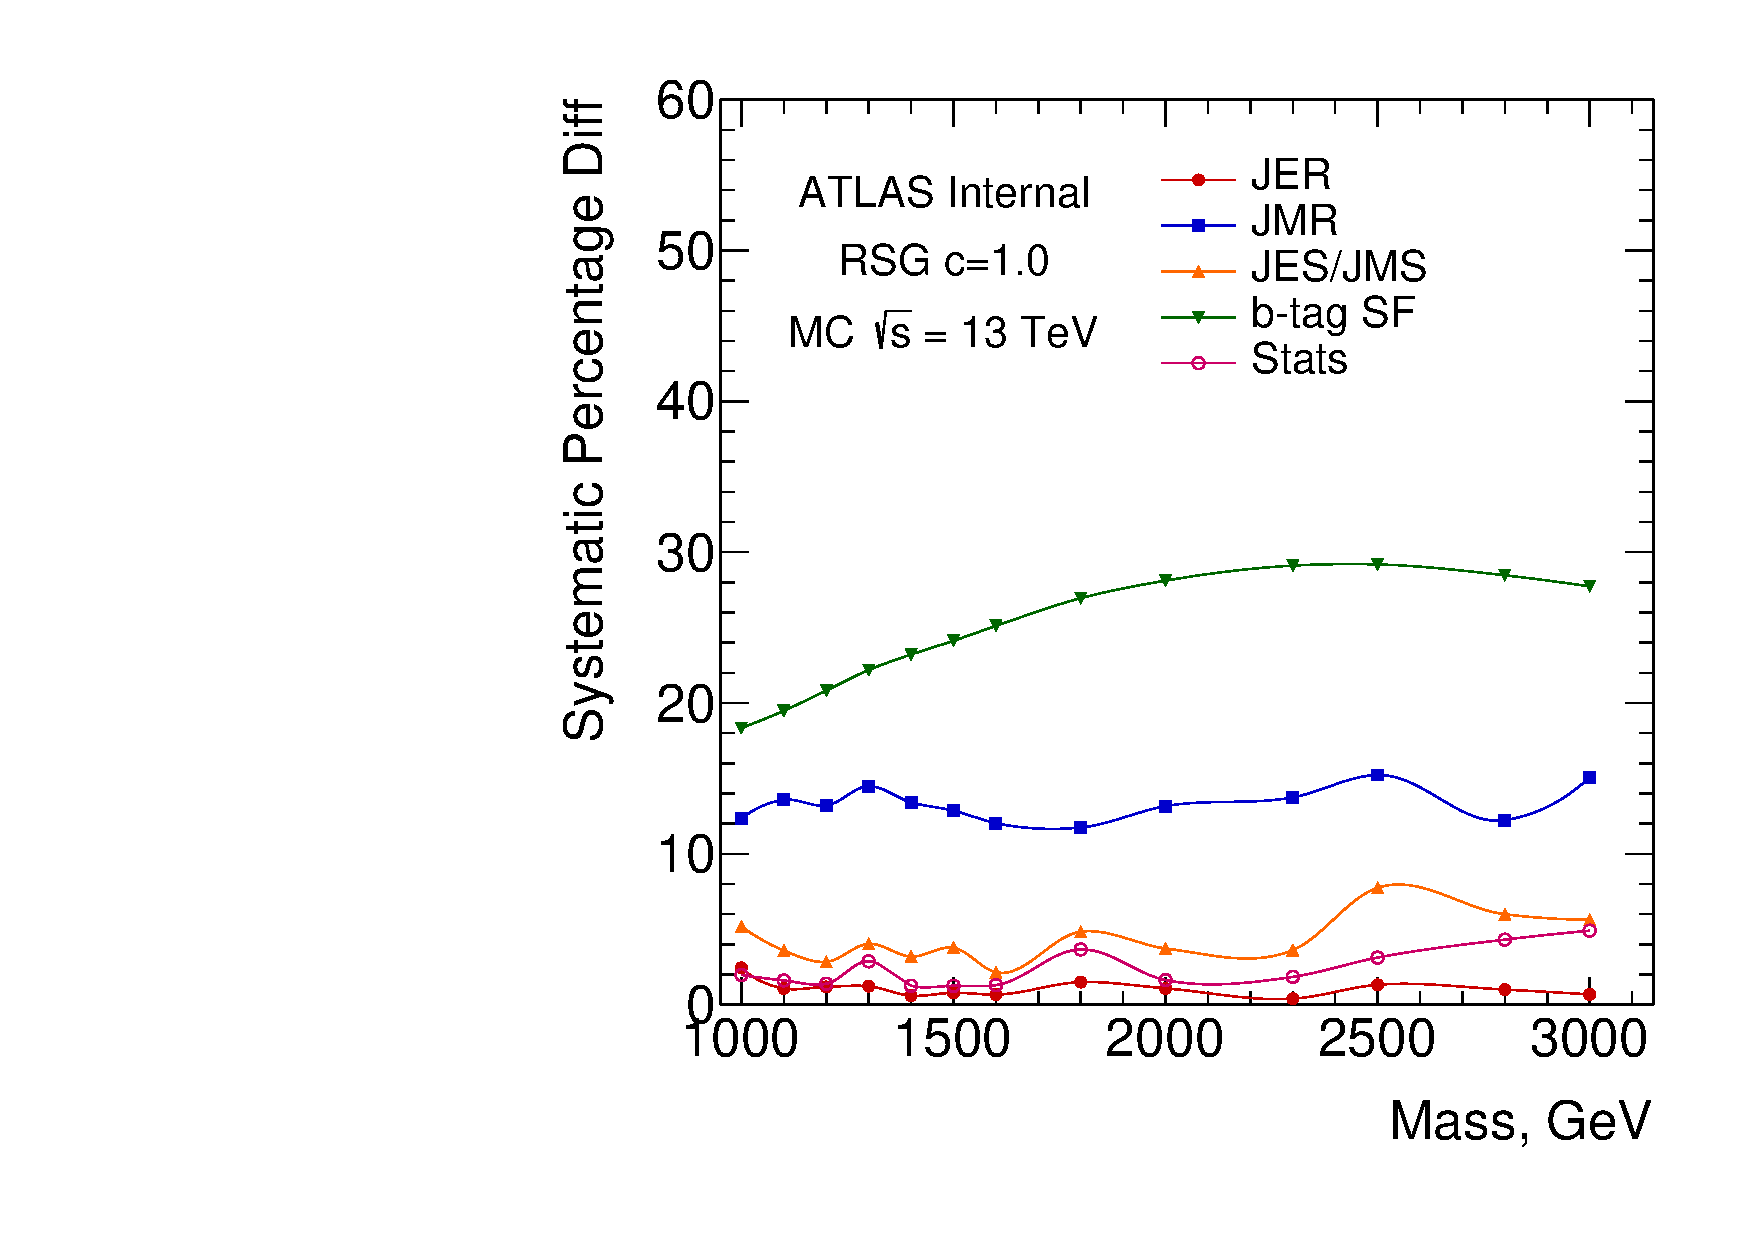
\includegraphics[angle=270, width=0.31\textwidth]{figures/boosted/Syst_MC/FourTag_RSG_syst.pdf}
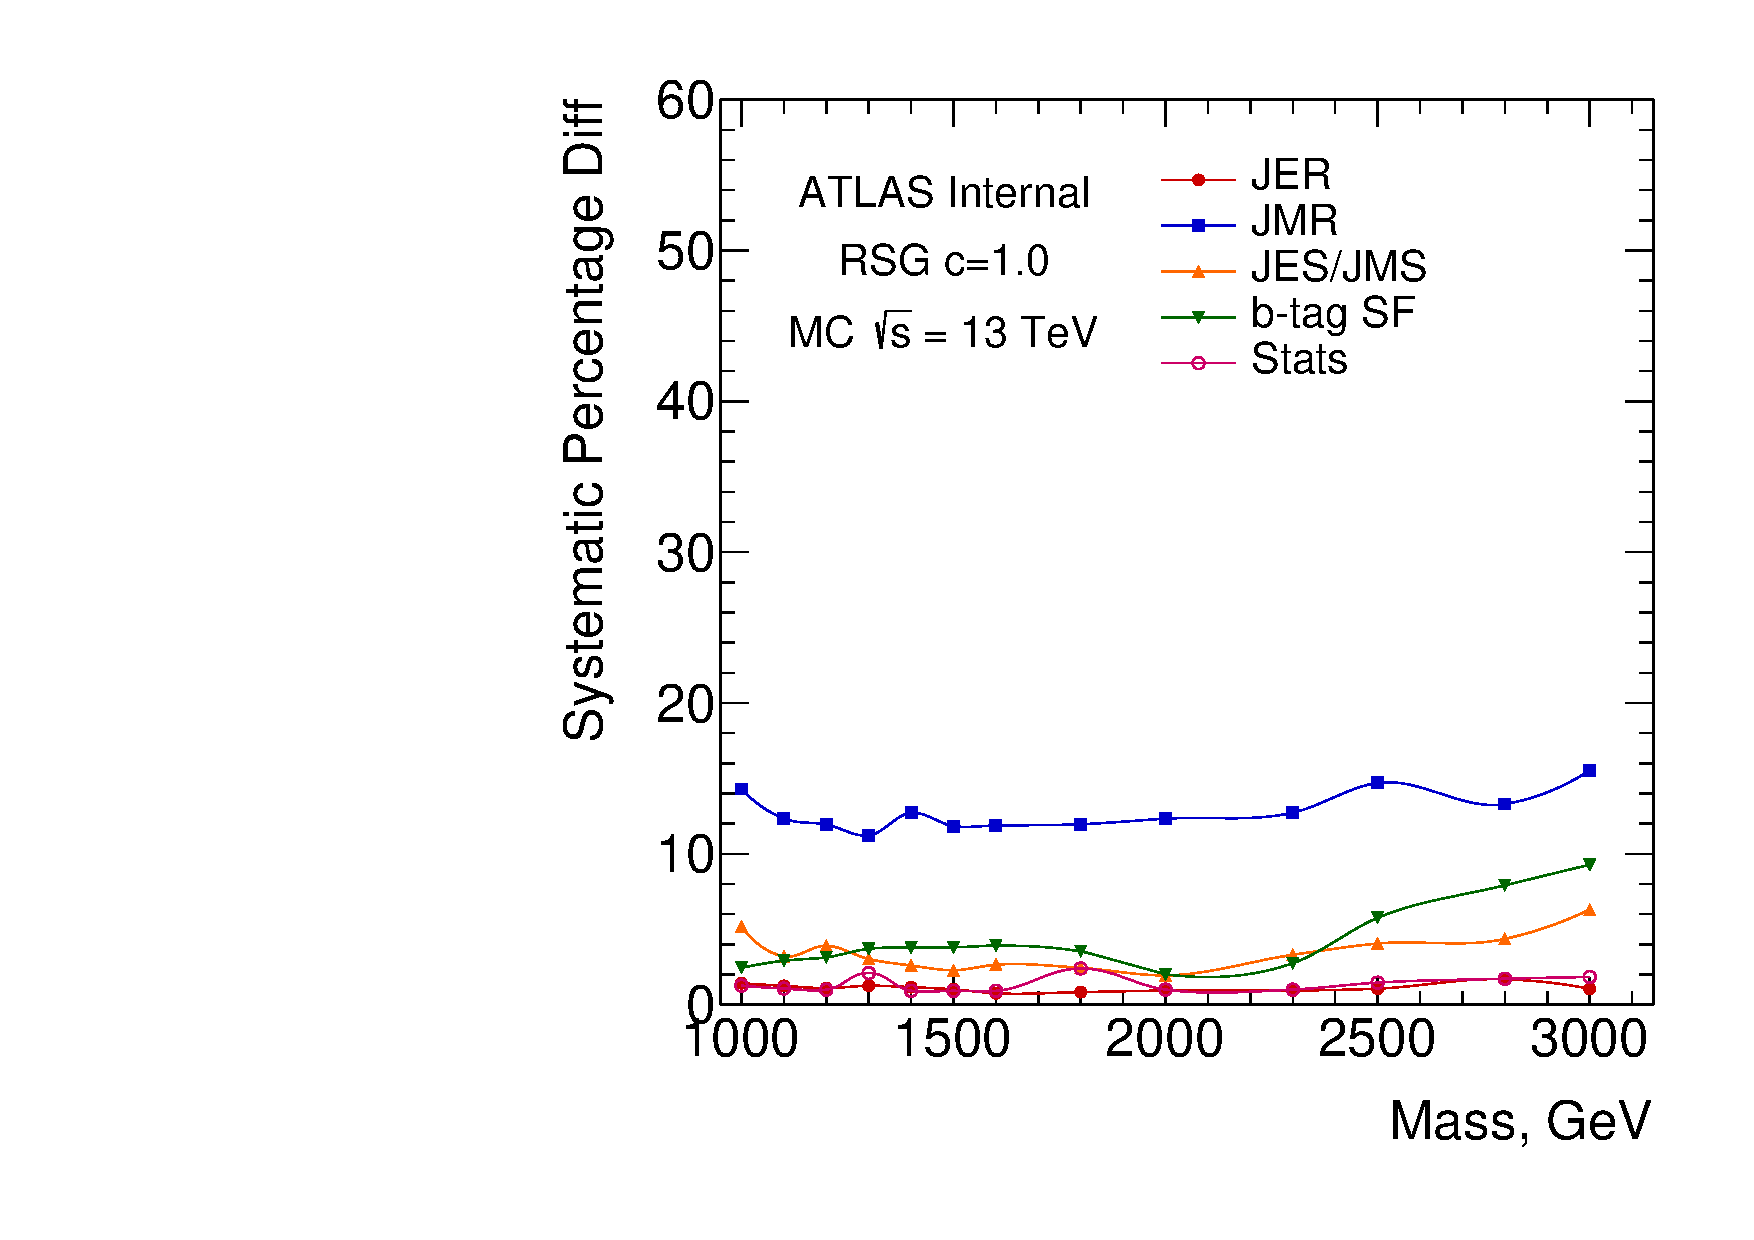
\includegraphics[angle=270, width=0.31\textwidth]{figures/boosted/Syst_MC/ThreeTag_RSG_syst.pdf}
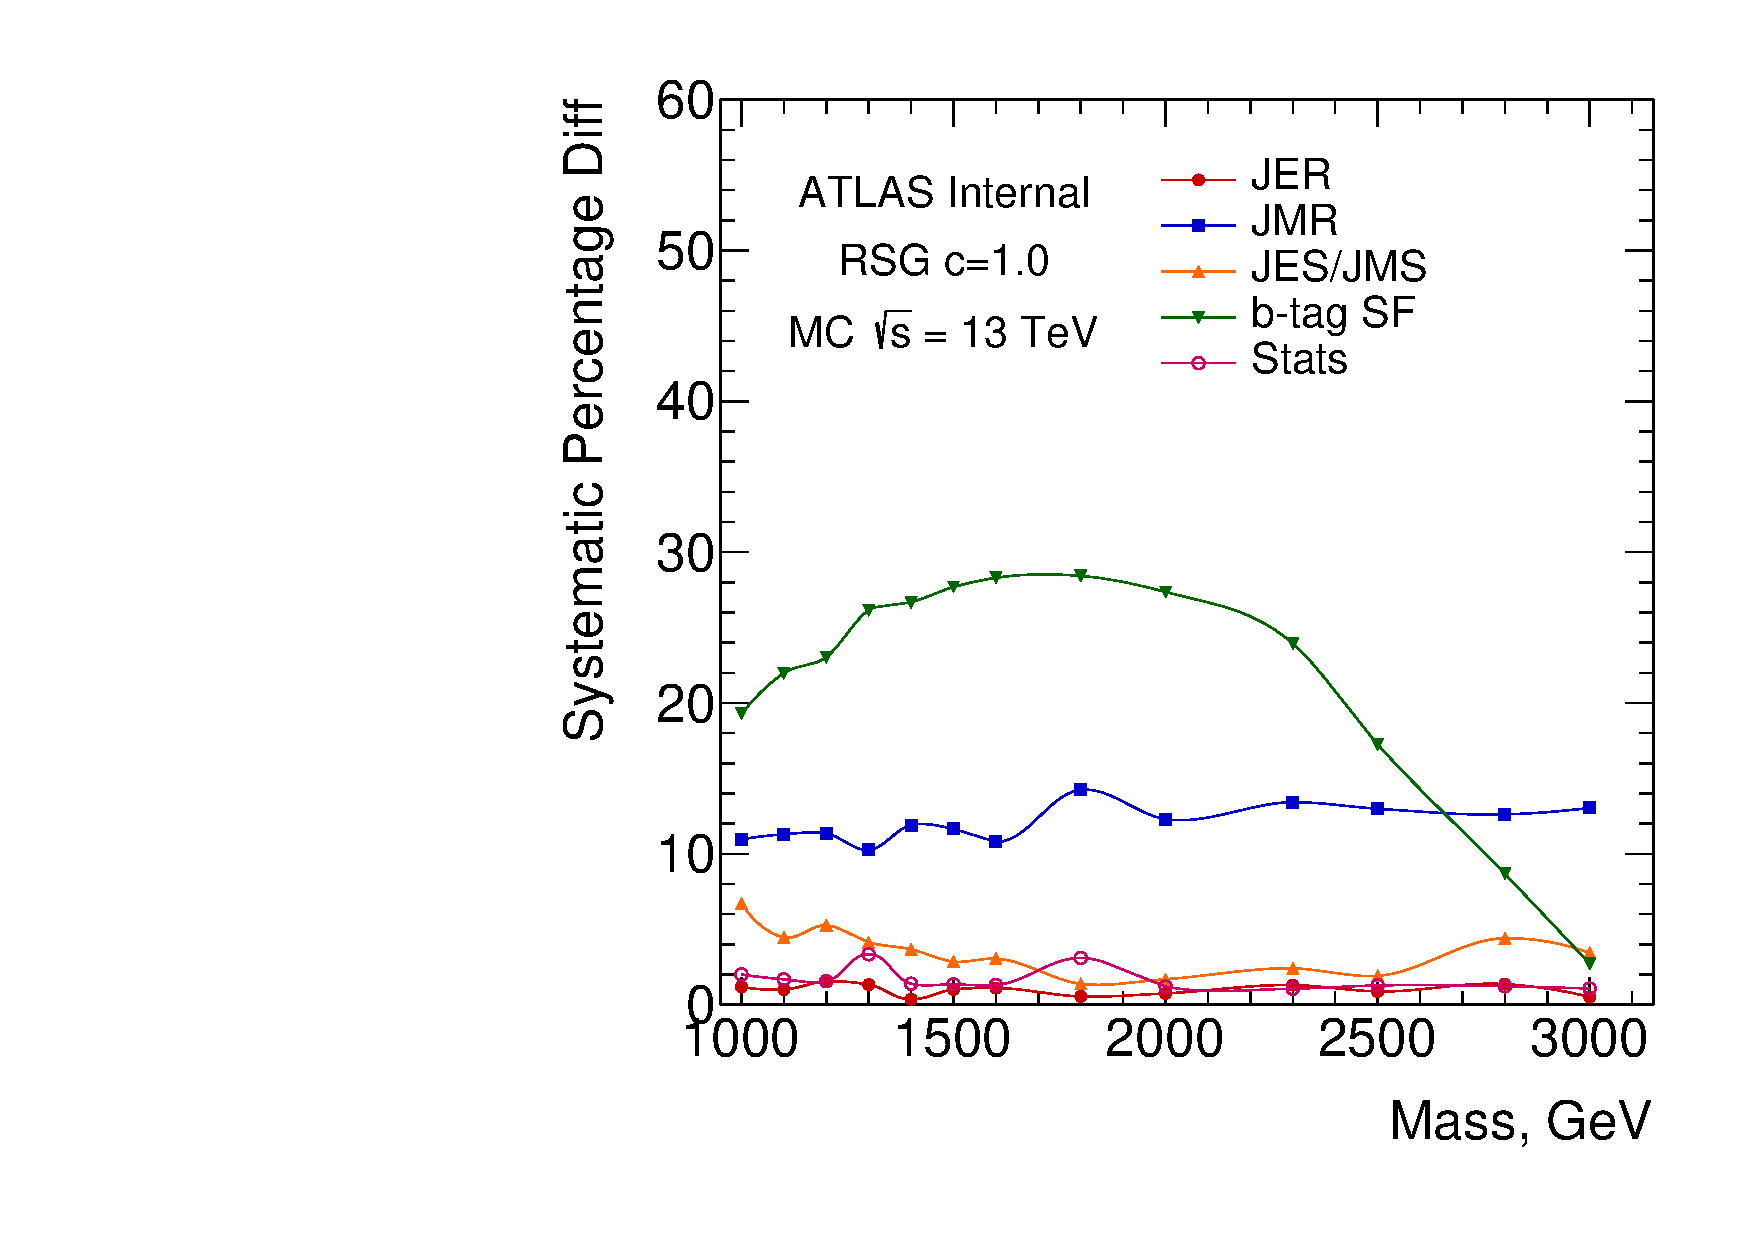
\includegraphics[angle=270, width=0.31\textwidth]{figures/boosted/Syst_MC/TwoTag_split_RSG_syst.pdf}
\caption{Impact of each systematic on the signal prediction as a function of the signal mass, in the $4b$ (left) and $3b$ (middle) and 2$b$s signal regions.}
\label{fig:signal_syst_summary}
\end{center}
\end{figure}

\paragraph{}
The final background prediction of MJJ along with total systematic uncertainties can be found in Figure~\ref{fig:FinalBkg_sys-4b}, ~\ref{fig:FinalBkg_sys-3b}, and ~\ref{fig:FinalBkg_sys-2b}. The final background prediction of scaled MJJ along with total uncertainties can be found in Figure~\ref{fig:FinalBkg_sys-4b-pole}, ~\ref{fig:FinalBkg_sys-3b-pole}, and ~\ref{fig:FinalBkg_sys-2b-pole}.


\begin{figure}
\begin{center}
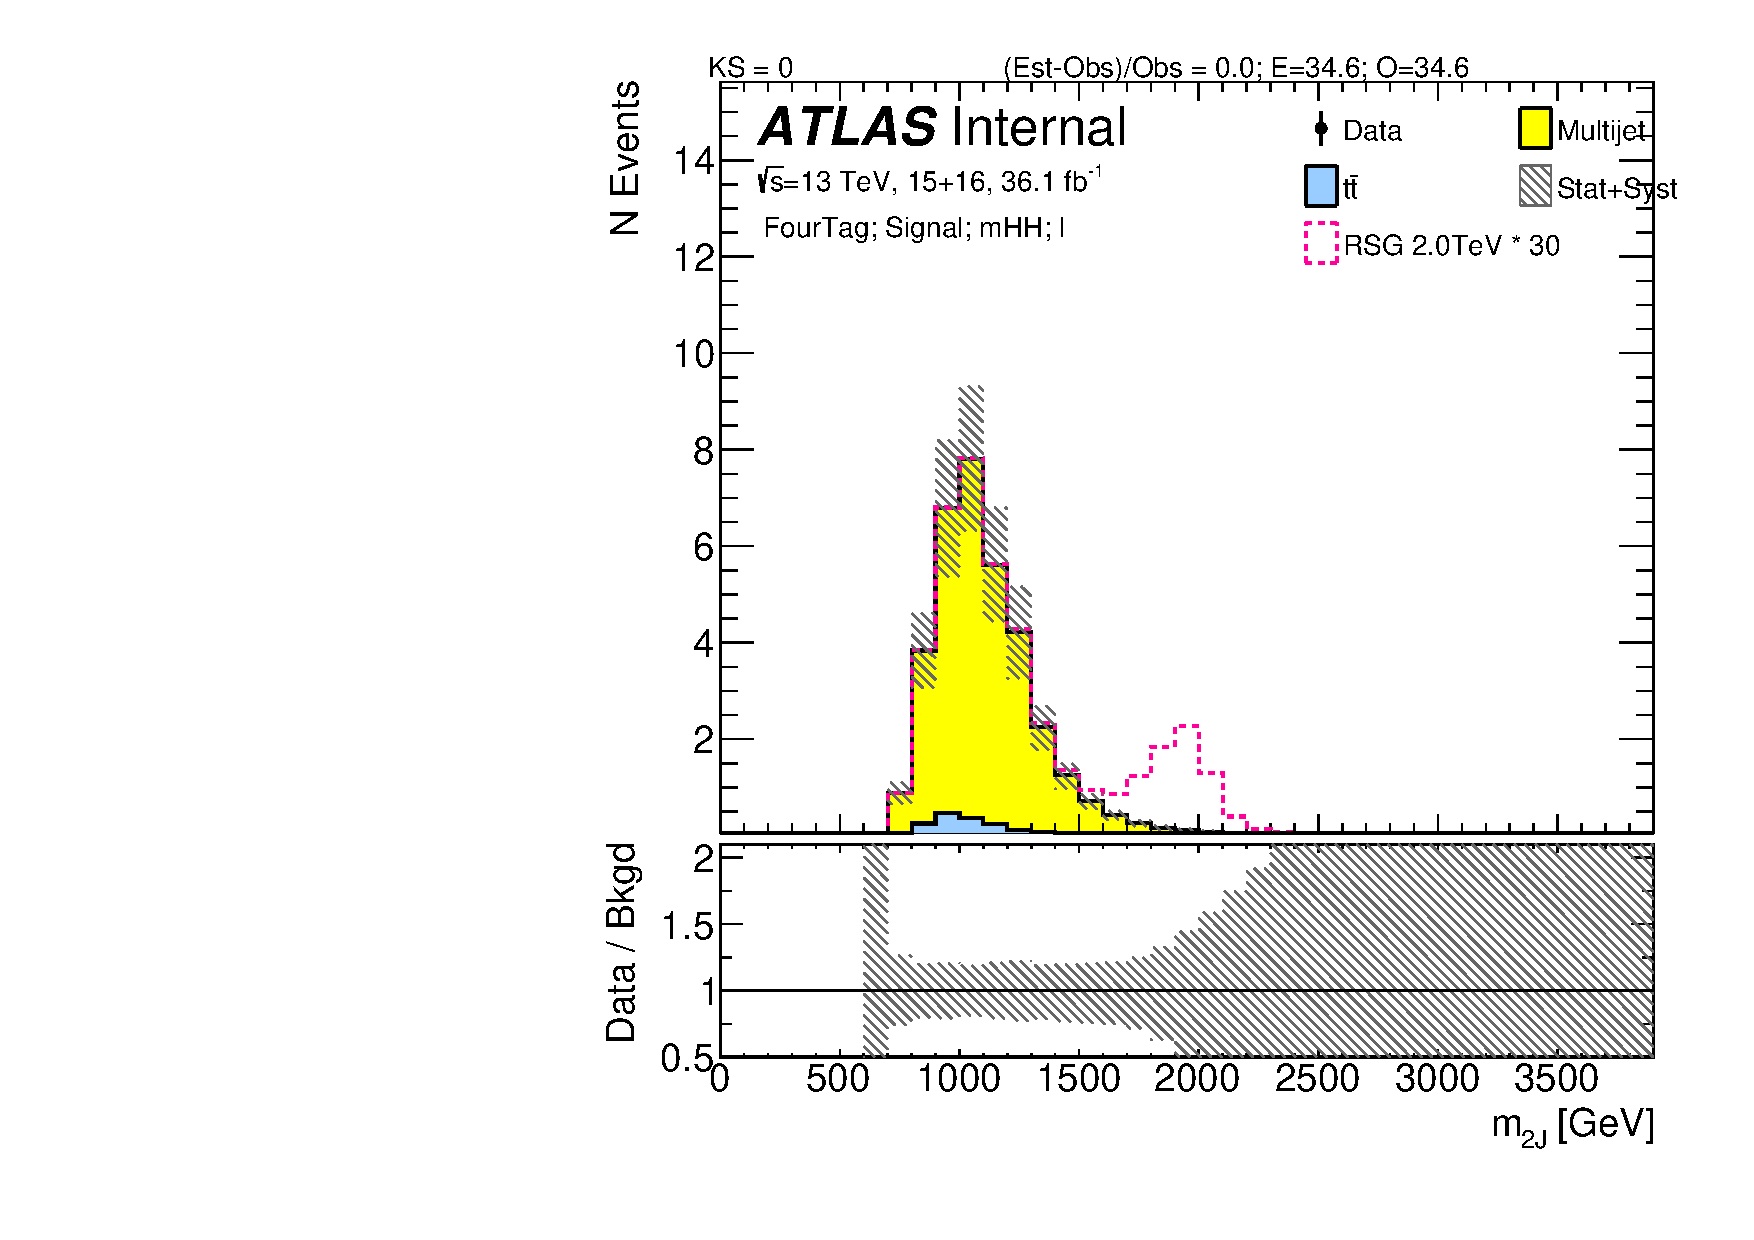
\includegraphics[angle=270, width=0.48\textwidth]{./figures/boosted/Signal_Syst/Moriond_bkg_9_FourTag_Signal_mHH_l_blind.pdf}
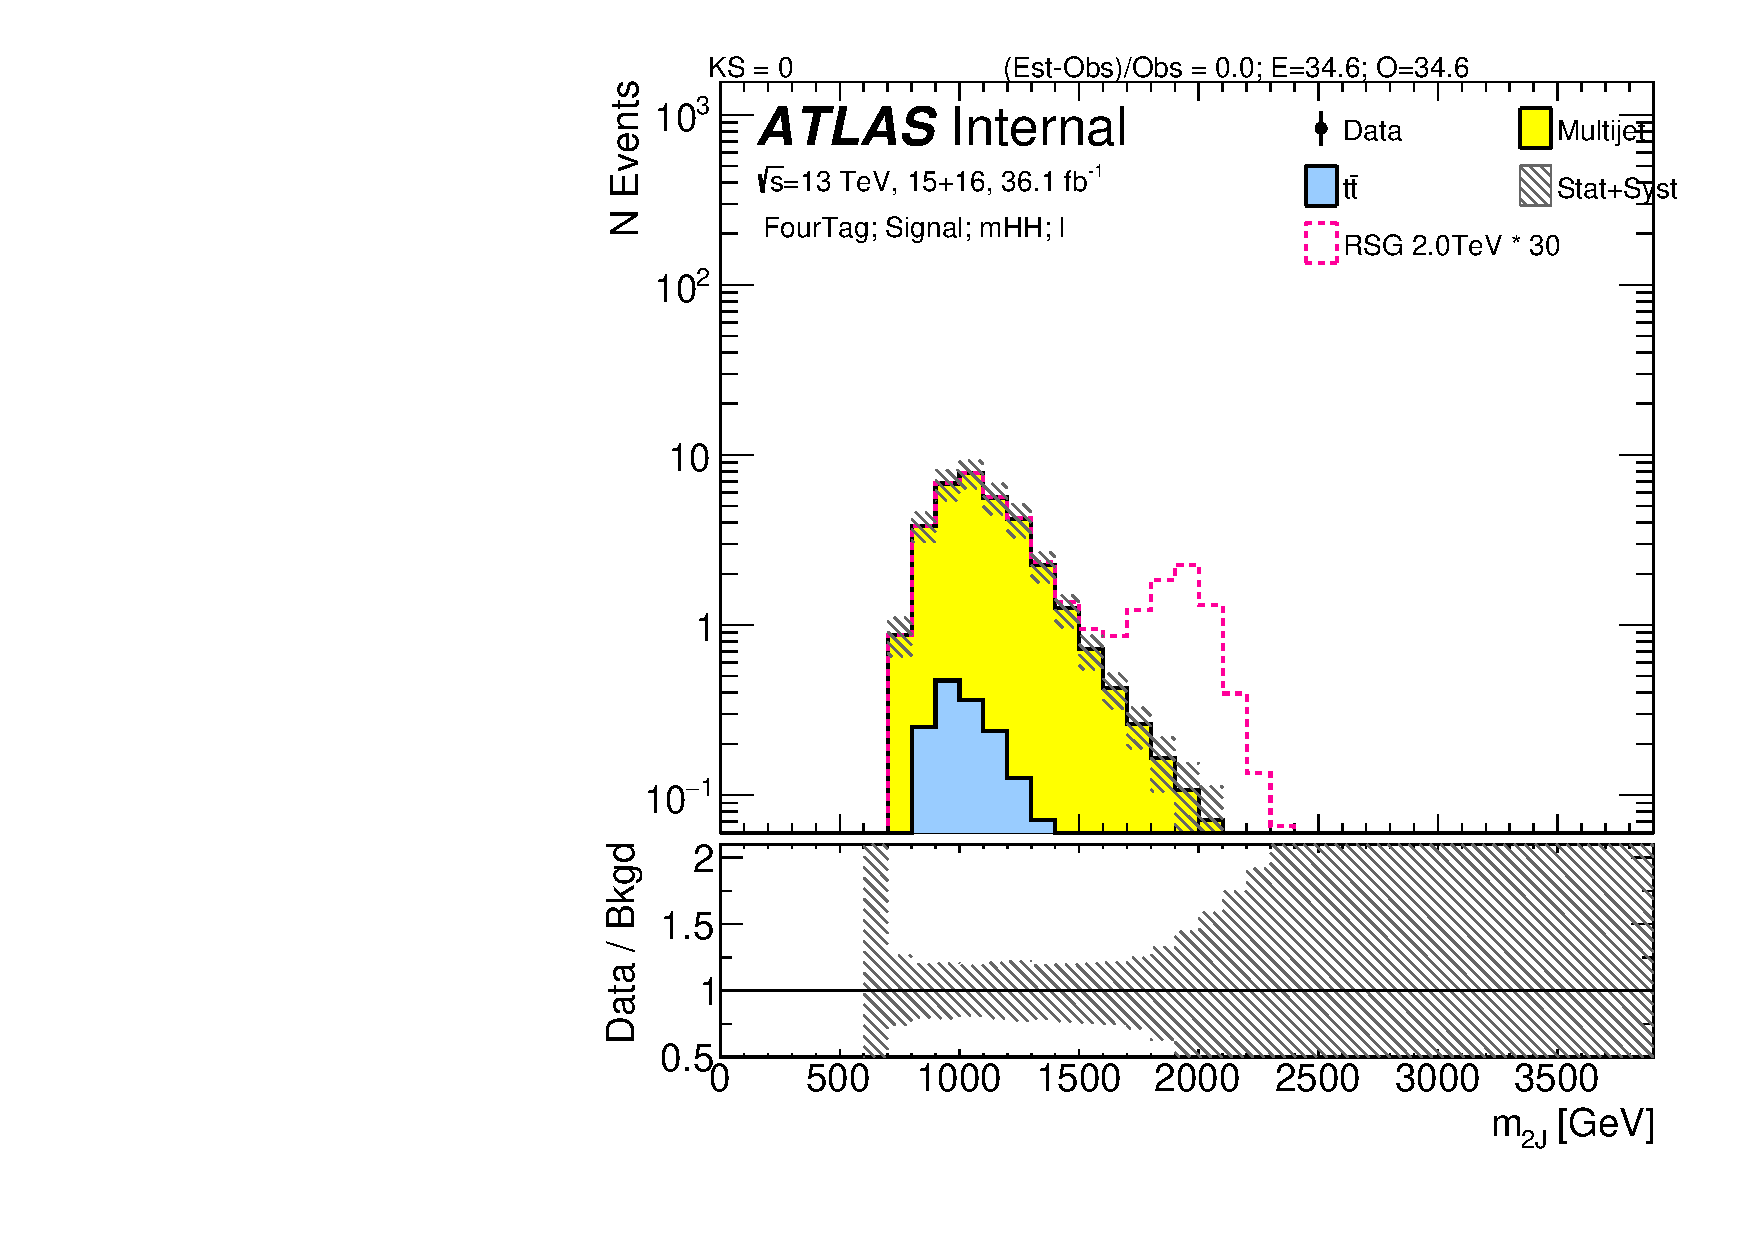
\includegraphics[angle=270, width=0.48\textwidth]{./figures/boosted/Signal_Syst/Moriond_bkg_9_FourTag_Signal_mHH_l_1_blind.pdf}
\caption{The total background estimation in $4b$ signal region, with linear scale on the left and with log scale on the right, along with total uncertainties (stats.$+$systematic) variation up and down.}
\label{fig:FinalBkg_sys-4b}
\end{center}
\end{figure}


\begin{figure}
\begin{center}
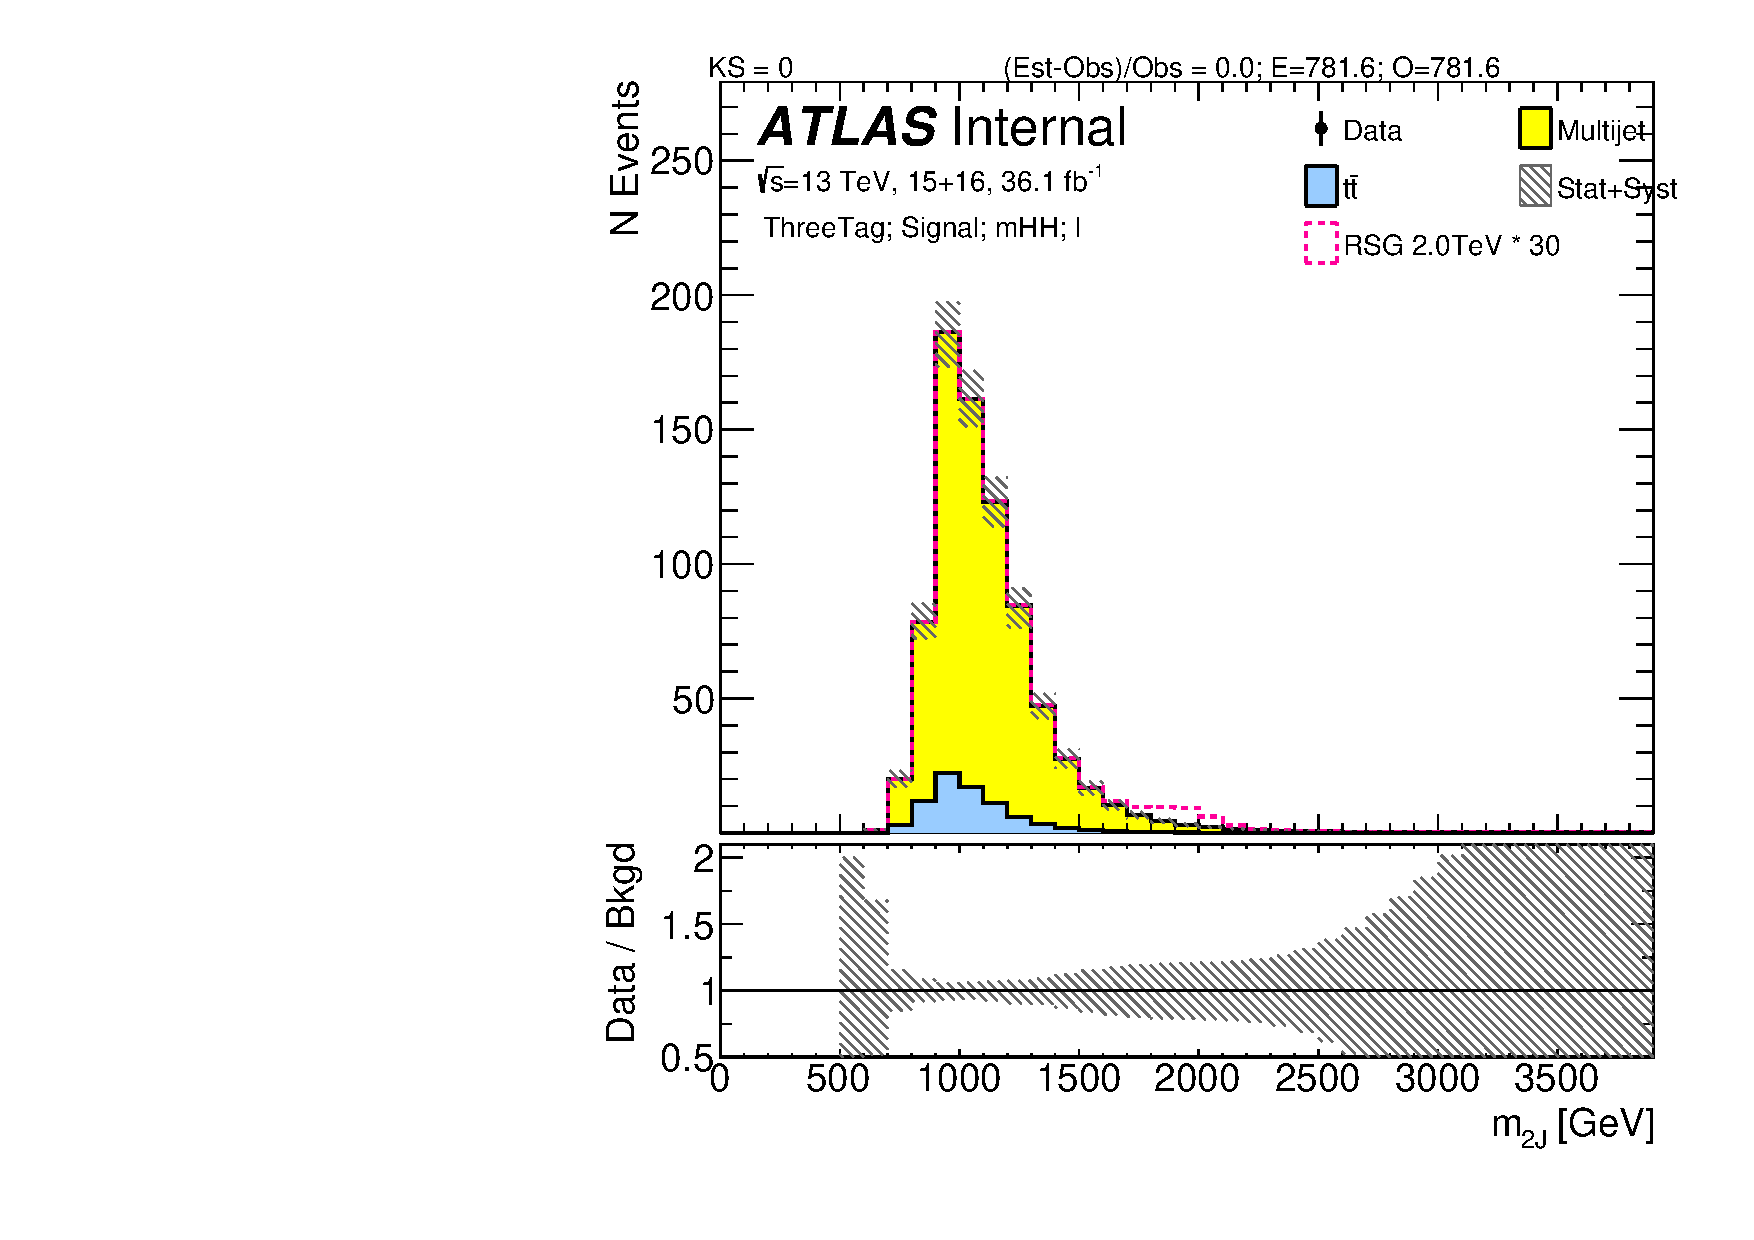
\includegraphics[angle=270, width=0.48\textwidth]{./figures/boosted/Signal_Syst/Moriond_bkg_9_ThreeTag_Signal_mHH_l_blind.pdf}
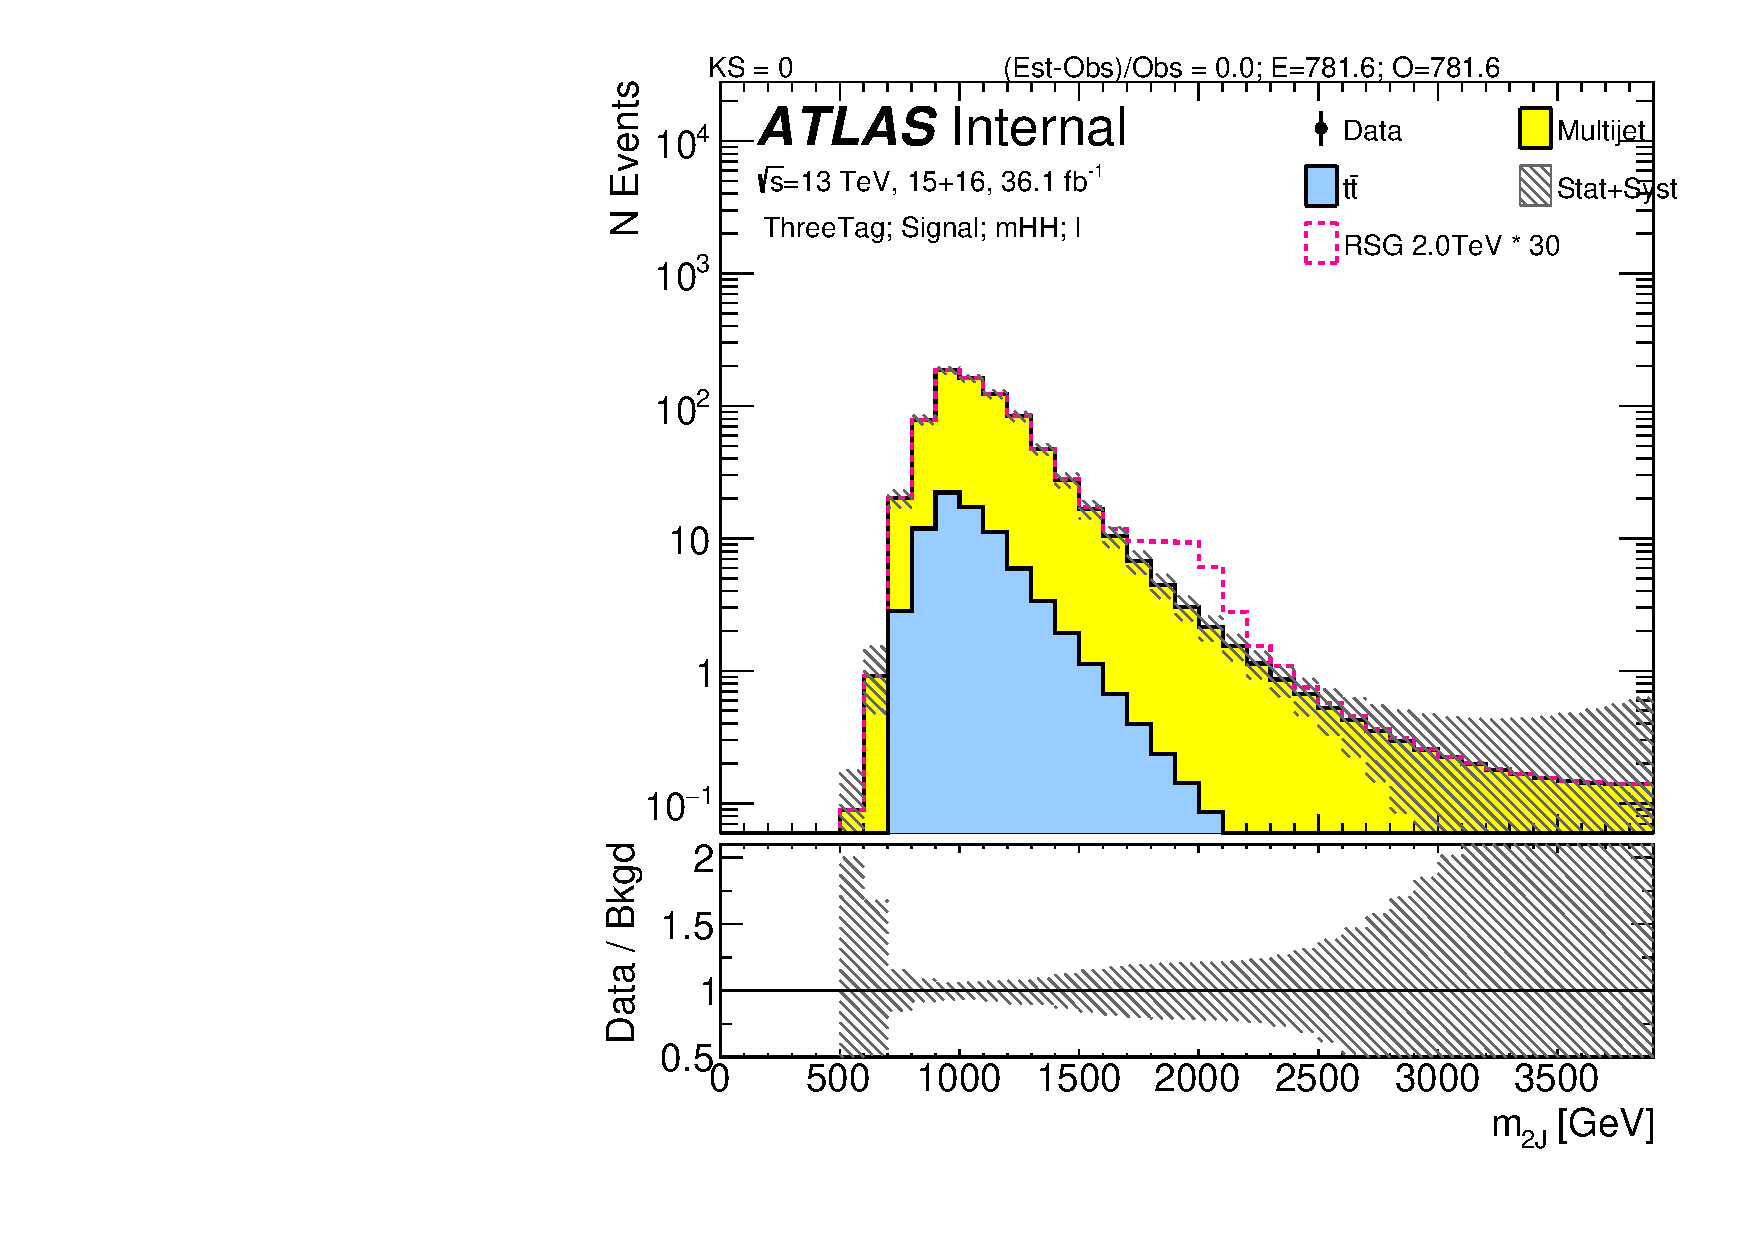
\includegraphics[angle=270, width=0.48\textwidth]{./figures/boosted/Signal_Syst/Moriond_bkg_9_ThreeTag_Signal_mHH_l_1_blind.pdf}
\caption{The total background estimation in $3b$ signal region, with linear scale on the left and with log scale on the right, along with total uncertainties (stats.$+$systematic) variation up and down.}
\label{fig:FinalBkg_sys-3b}
\end{center}
\end{figure}


\begin{figure}
\begin{center}
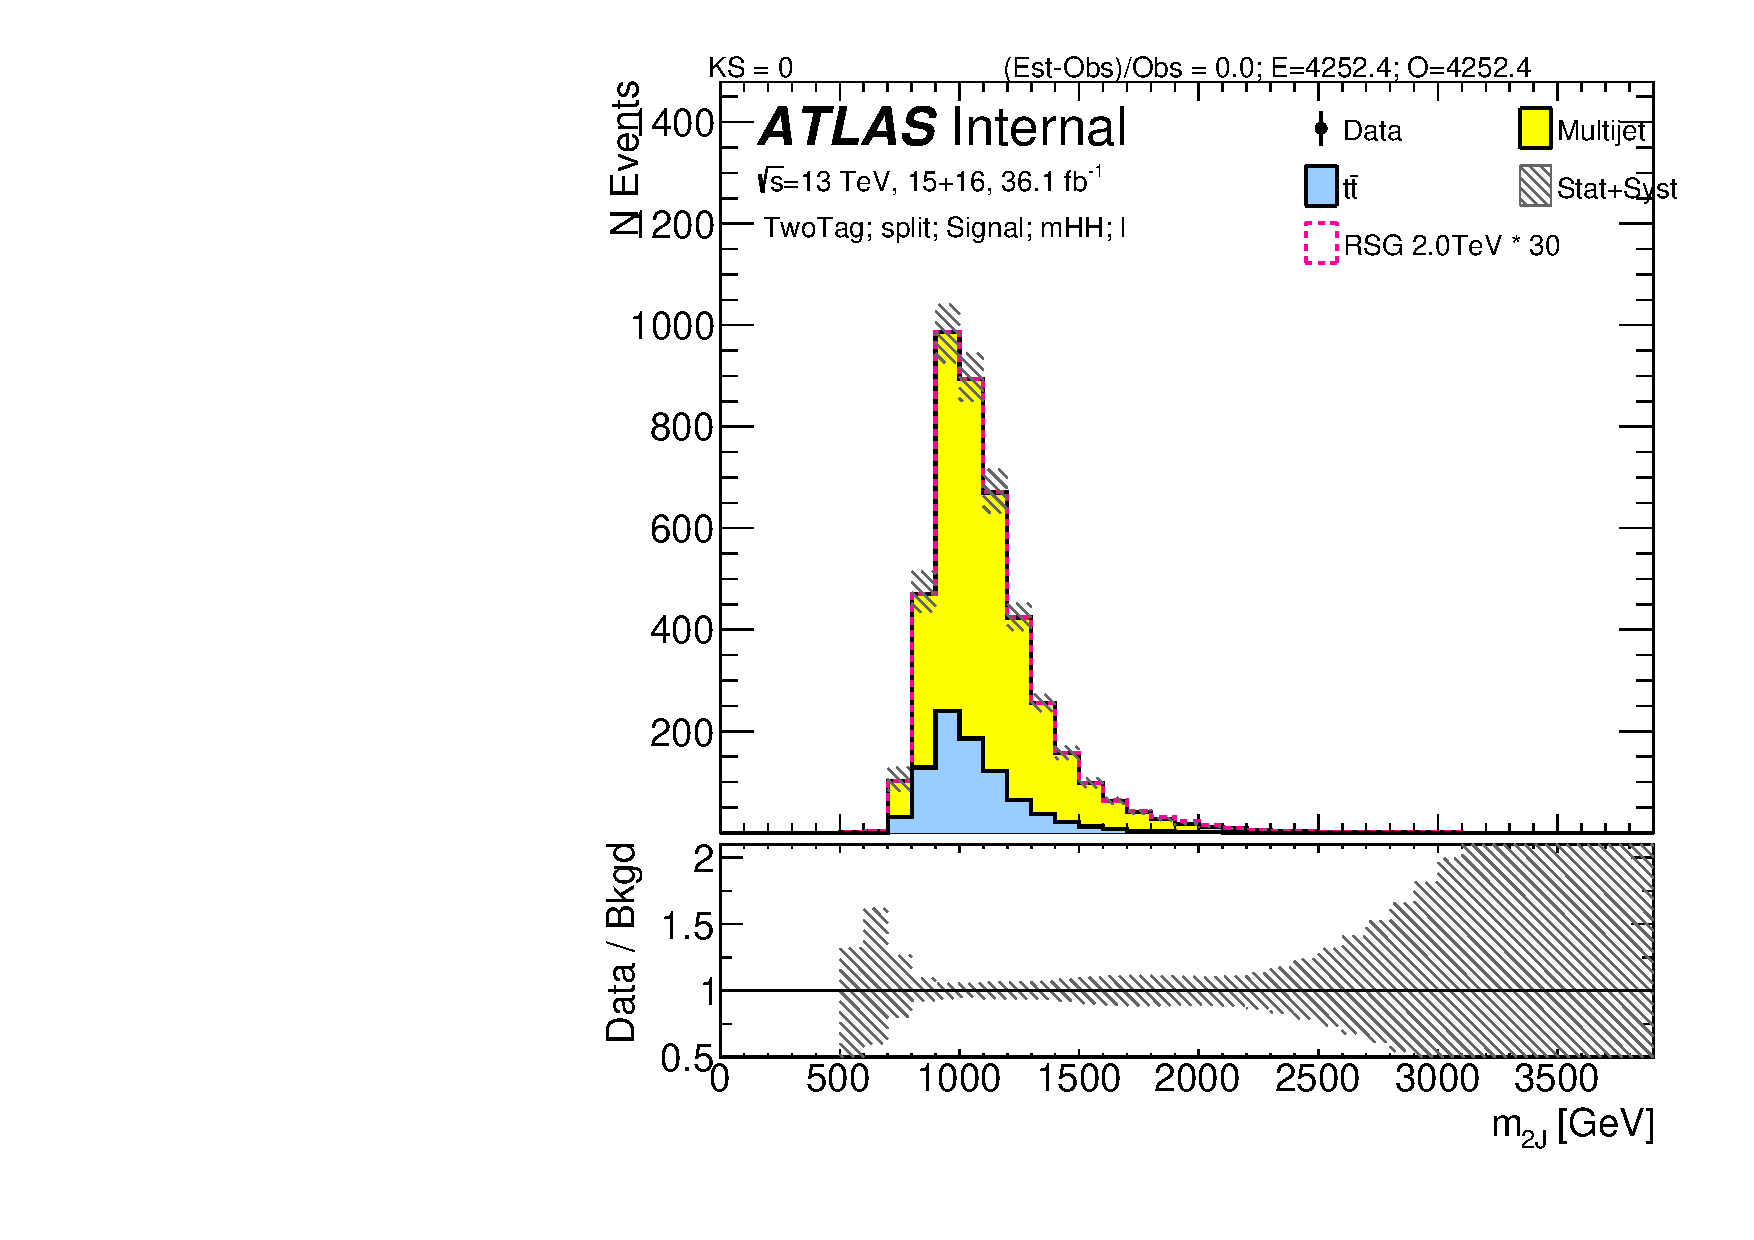
\includegraphics[angle=270, width=0.48\textwidth]{./figures/boosted/Signal_Syst/Moriond_bkg_9_TwoTag_split_Signal_mHH_l_blind.pdf}
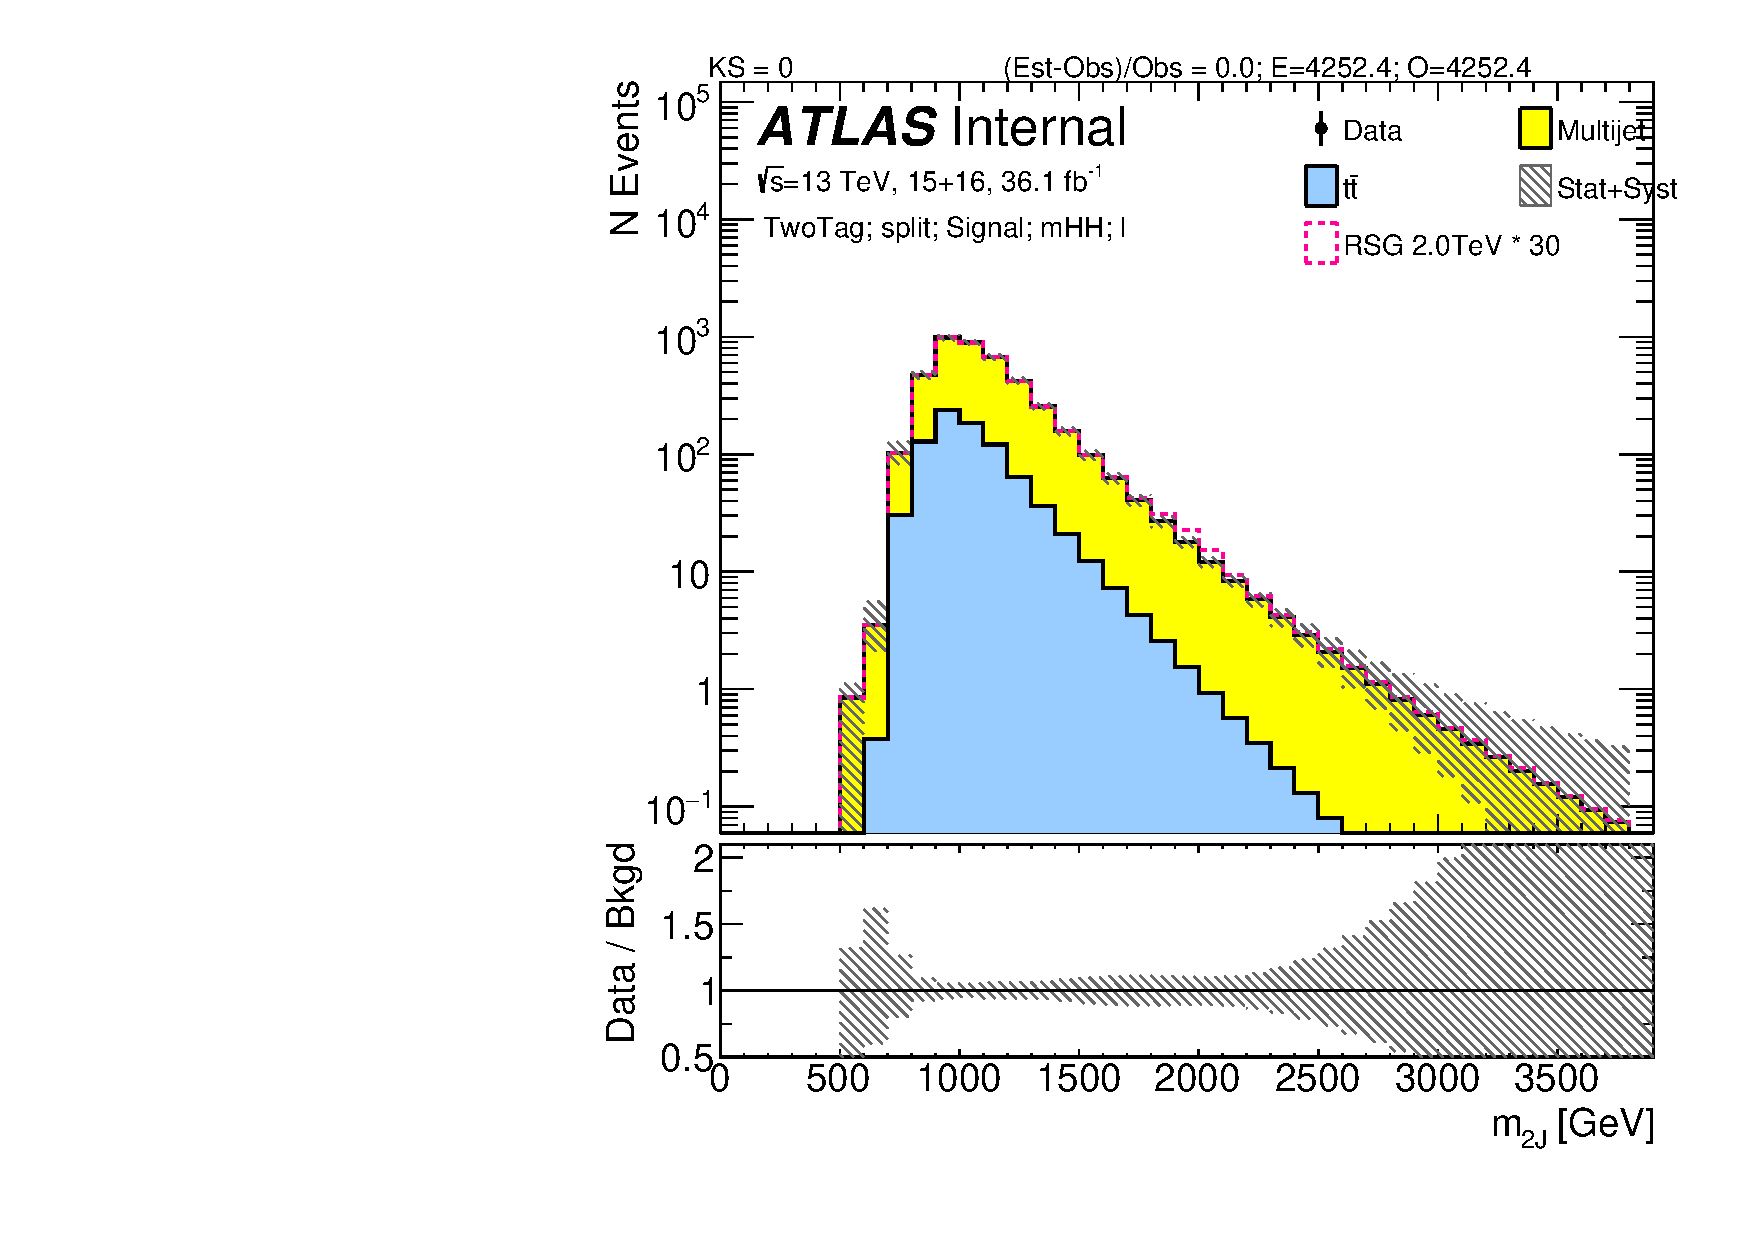
\includegraphics[angle=270, width=0.48\textwidth]{./figures/boosted/Signal_Syst/Moriond_bkg_9_TwoTag_split_Signal_mHH_l_1_blind.pdf}
\caption{The total background estimation in $2b$s signal region, with linear scale on the left and with log scale on the right, along with total uncertainties (stats.$+$systematic) variation up and down.}
\label{fig:FinalBkg_sys-2b}
\end{center}
\end{figure}

\begin{figure}
\begin{center}
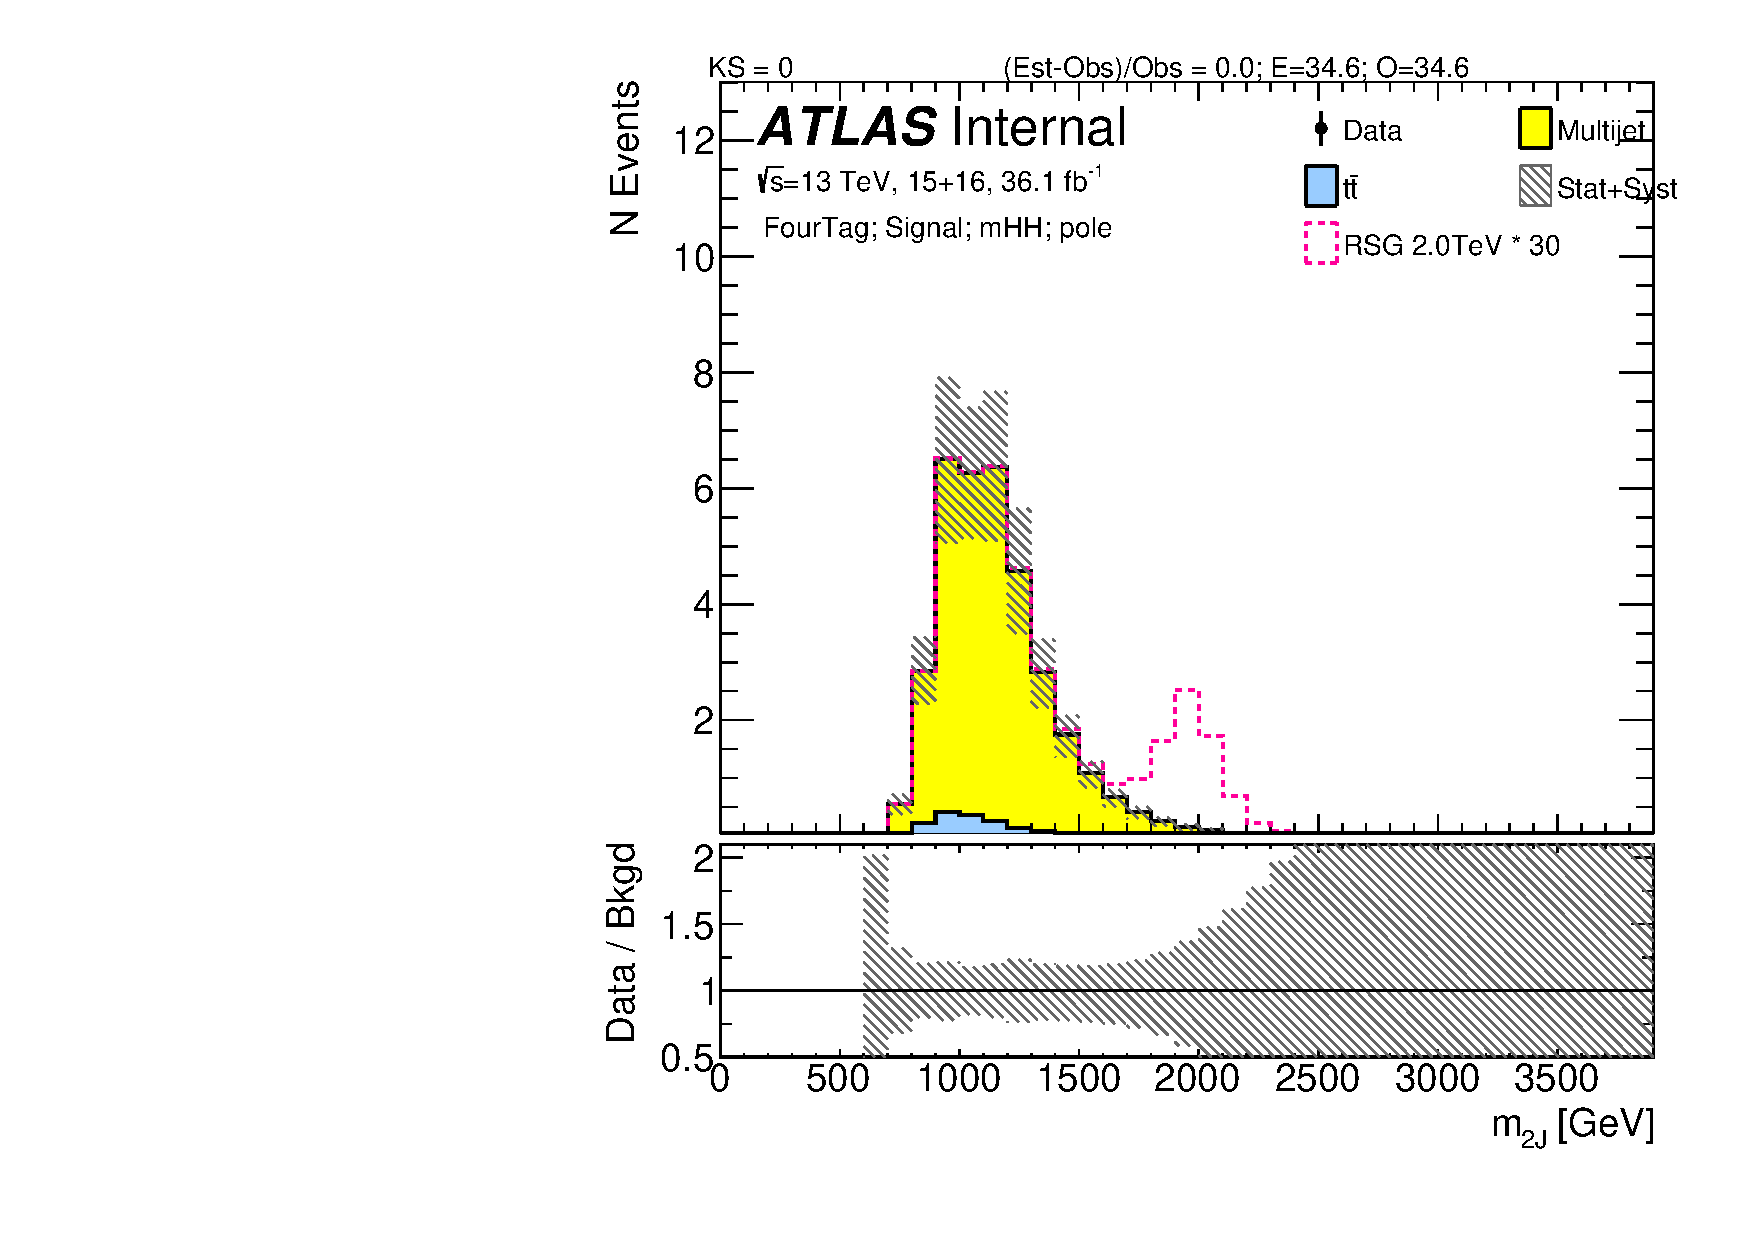
\includegraphics[angle=270, width=0.48\textwidth]{./figures/boosted/Signal_Syst/Moriond_bkg_9_FourTag_Signal_mHH_pole_blind.pdf}
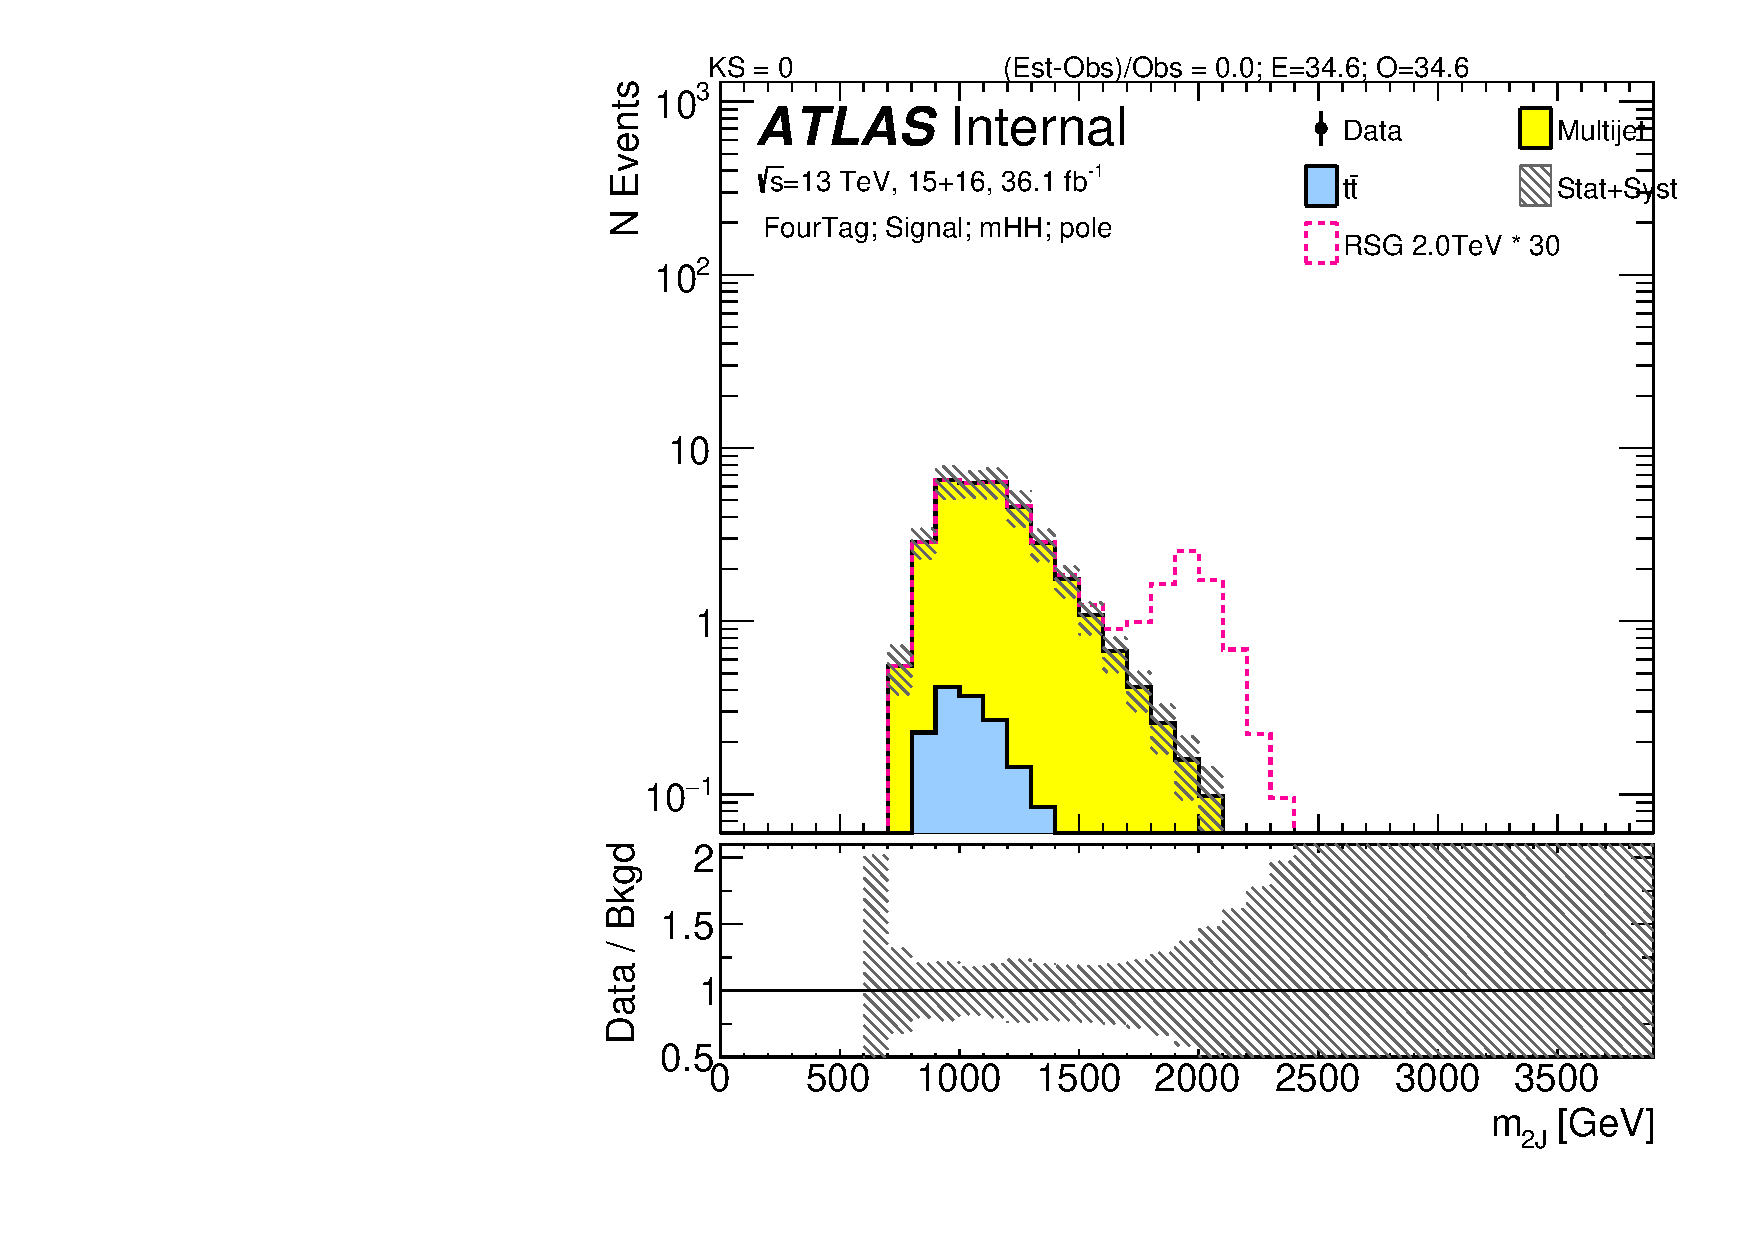
\includegraphics[angle=270, width=0.48\textwidth]{./figures/boosted/Signal_Syst/Moriond_bkg_9_FourTag_Signal_mHH_pole_1_blind.pdf}
\caption{The total background estimation in $4b$ signal region, scaled mJJ, with linear scale on the left and with log scale on the right, along with total uncertainties (stats.$+$systematic) variation up and down.}
\label{fig:FinalBkg_sys-4b-pole}
\end{center}
\end{figure}


\begin{figure}
\begin{center}
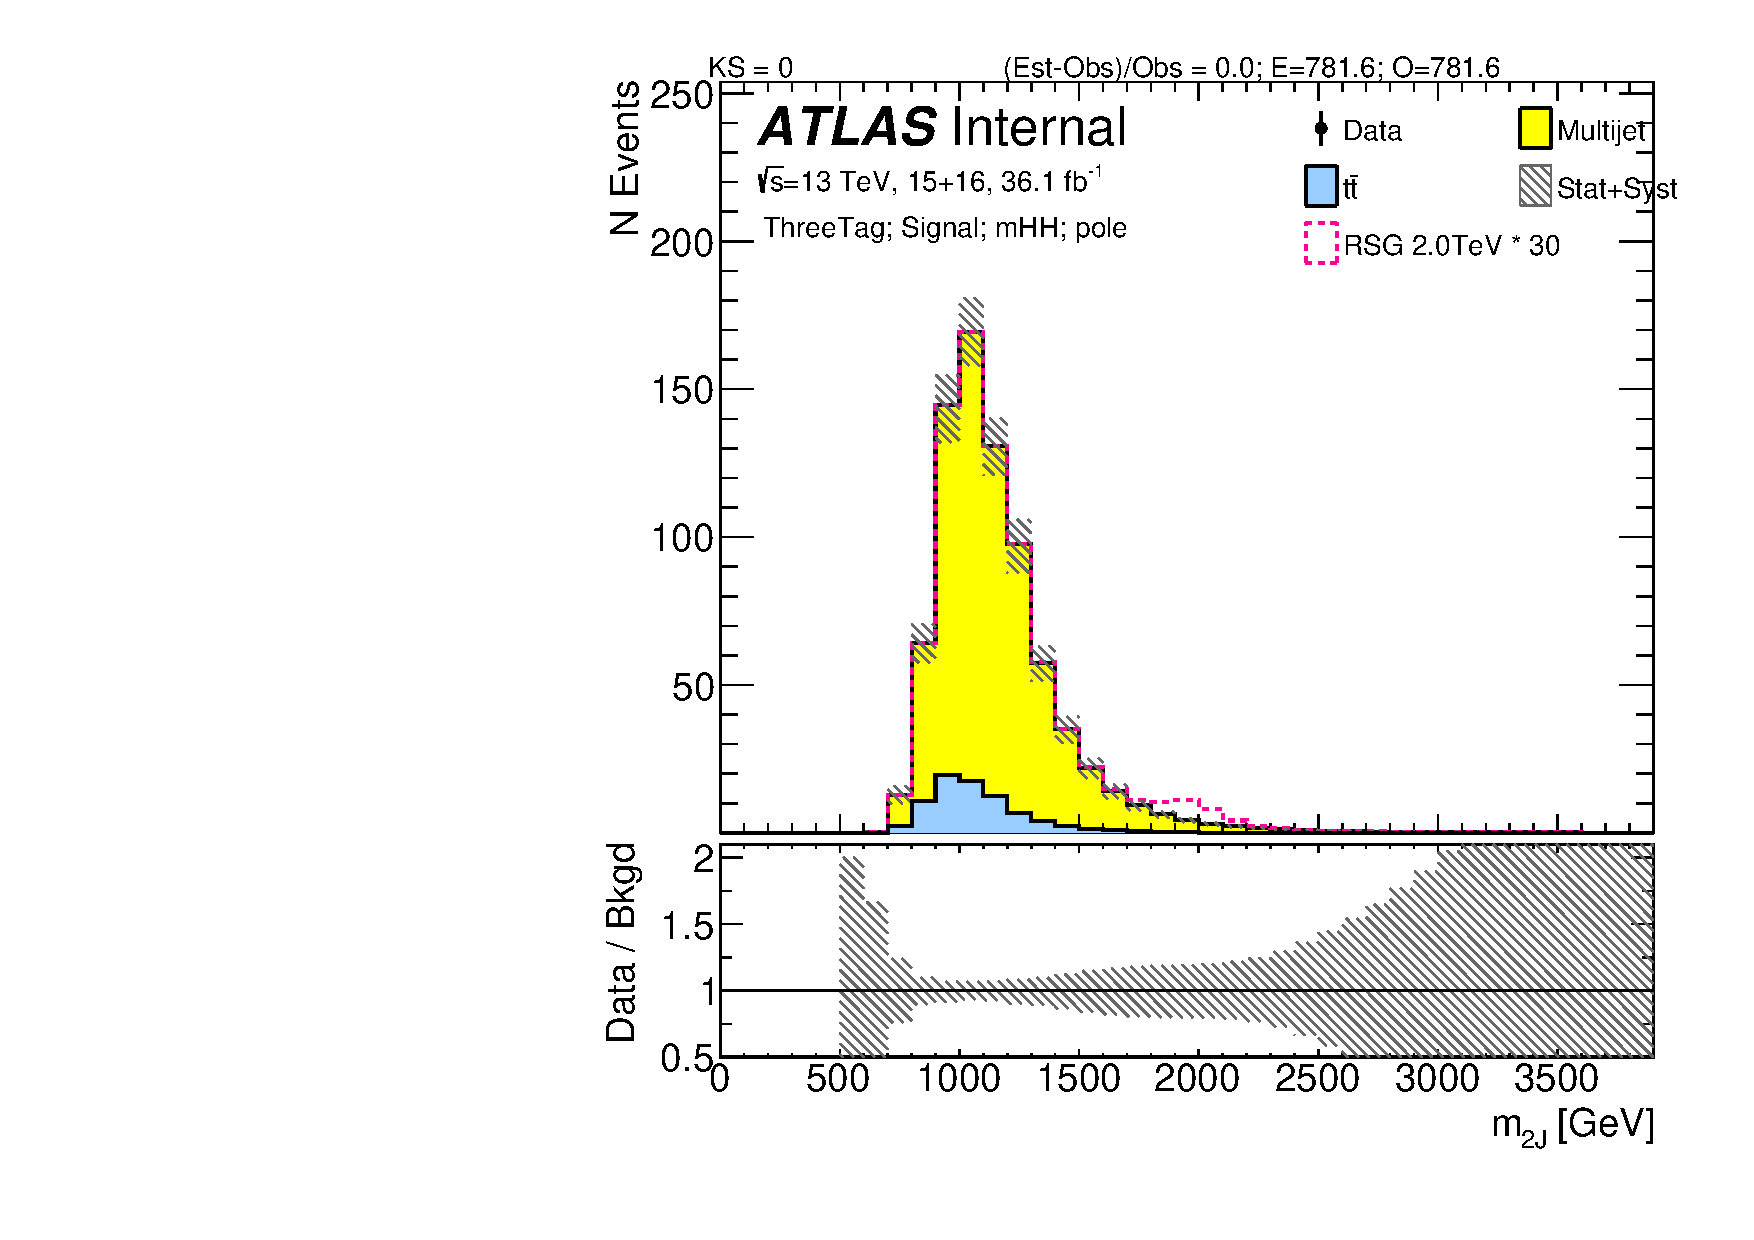
\includegraphics[angle=270, width=0.48\textwidth]{./figures/boosted/Signal_Syst/Moriond_bkg_9_ThreeTag_Signal_mHH_pole_blind.pdf}
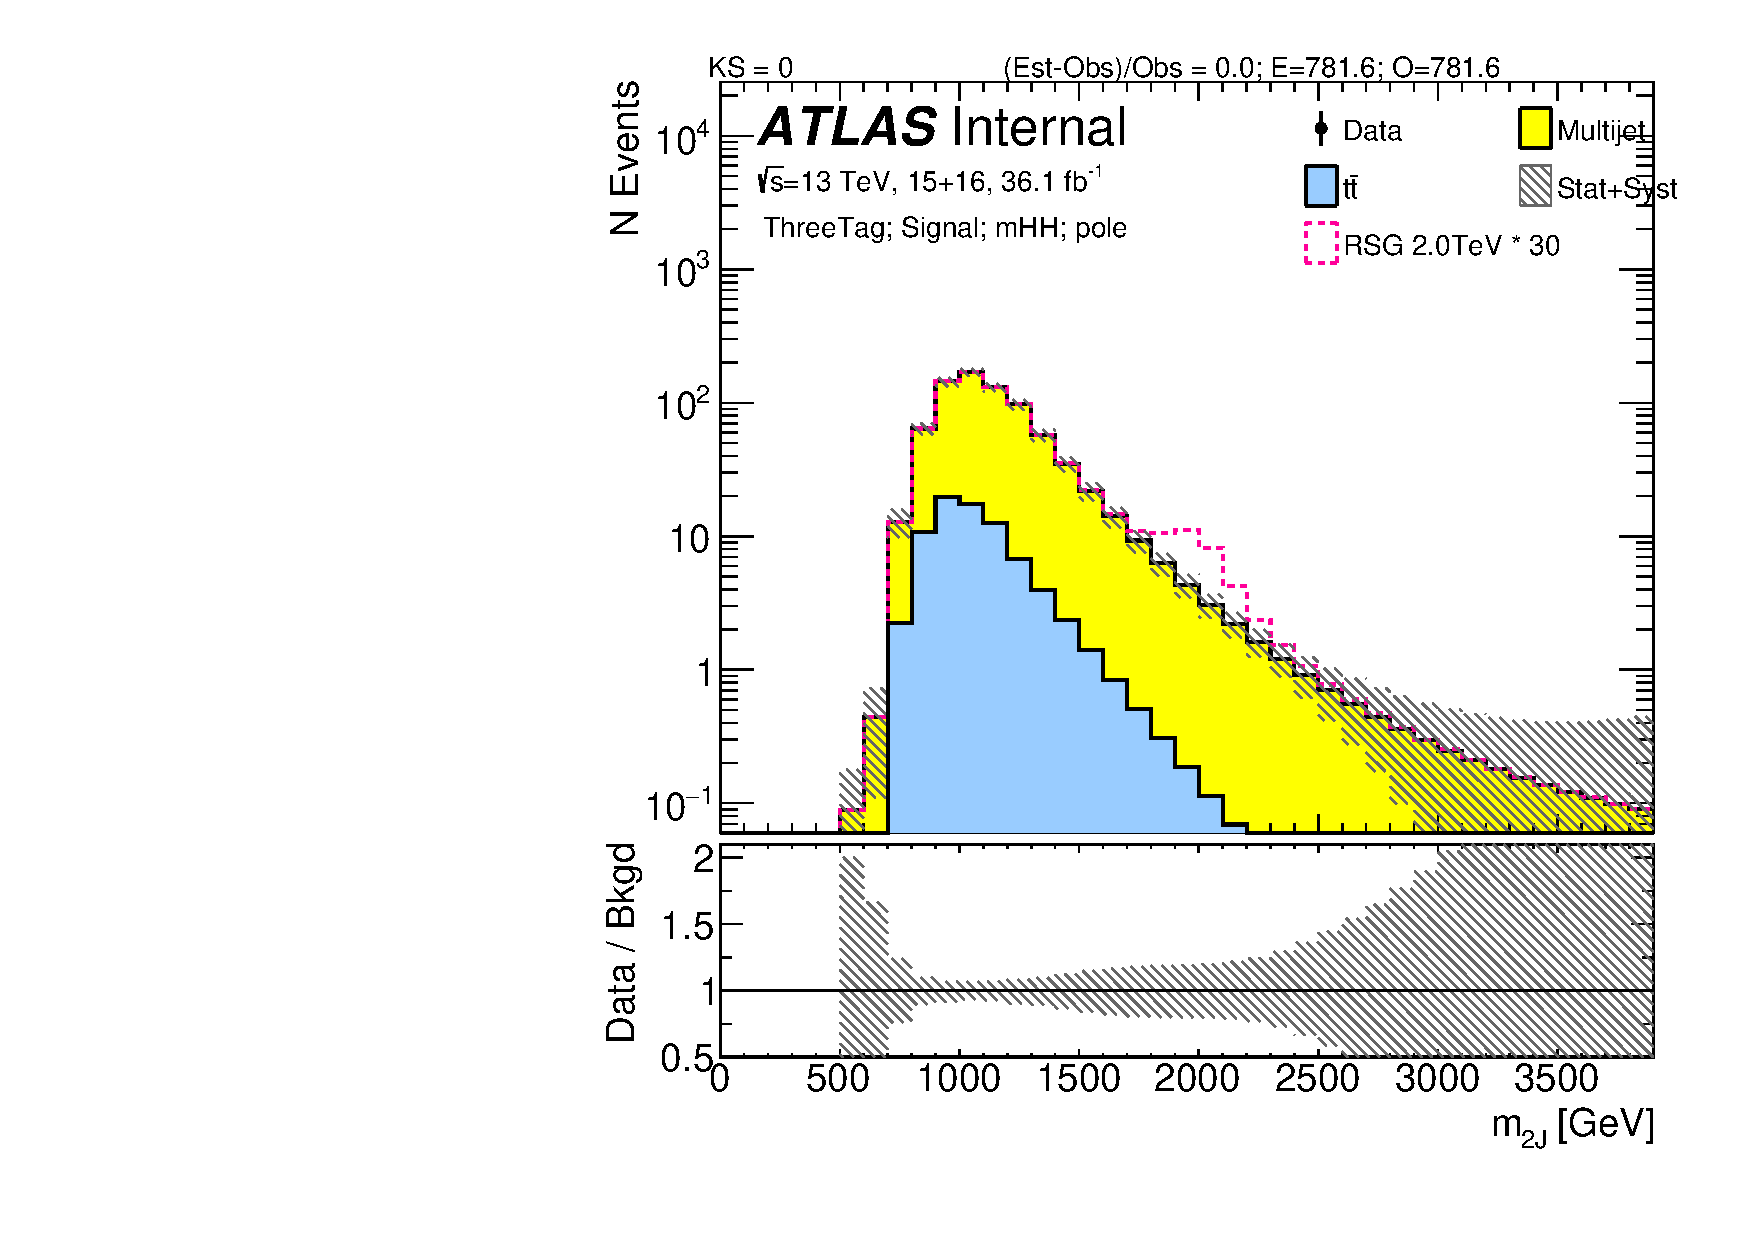
\includegraphics[angle=270, width=0.48\textwidth]{./figures/boosted/Signal_Syst/Moriond_bkg_9_ThreeTag_Signal_mHH_pole_1_blind.pdf}
\caption{The total background estimation in $3b$ signal region, scaled mJJ, with linear scale on the left and with log scale on the right, along with total uncertainties (stats.$+$systematic) variation up and down.}
\label{fig:FinalBkg_sys-3b-pole}
\end{center}
\end{figure}


\begin{figure}
\begin{center}
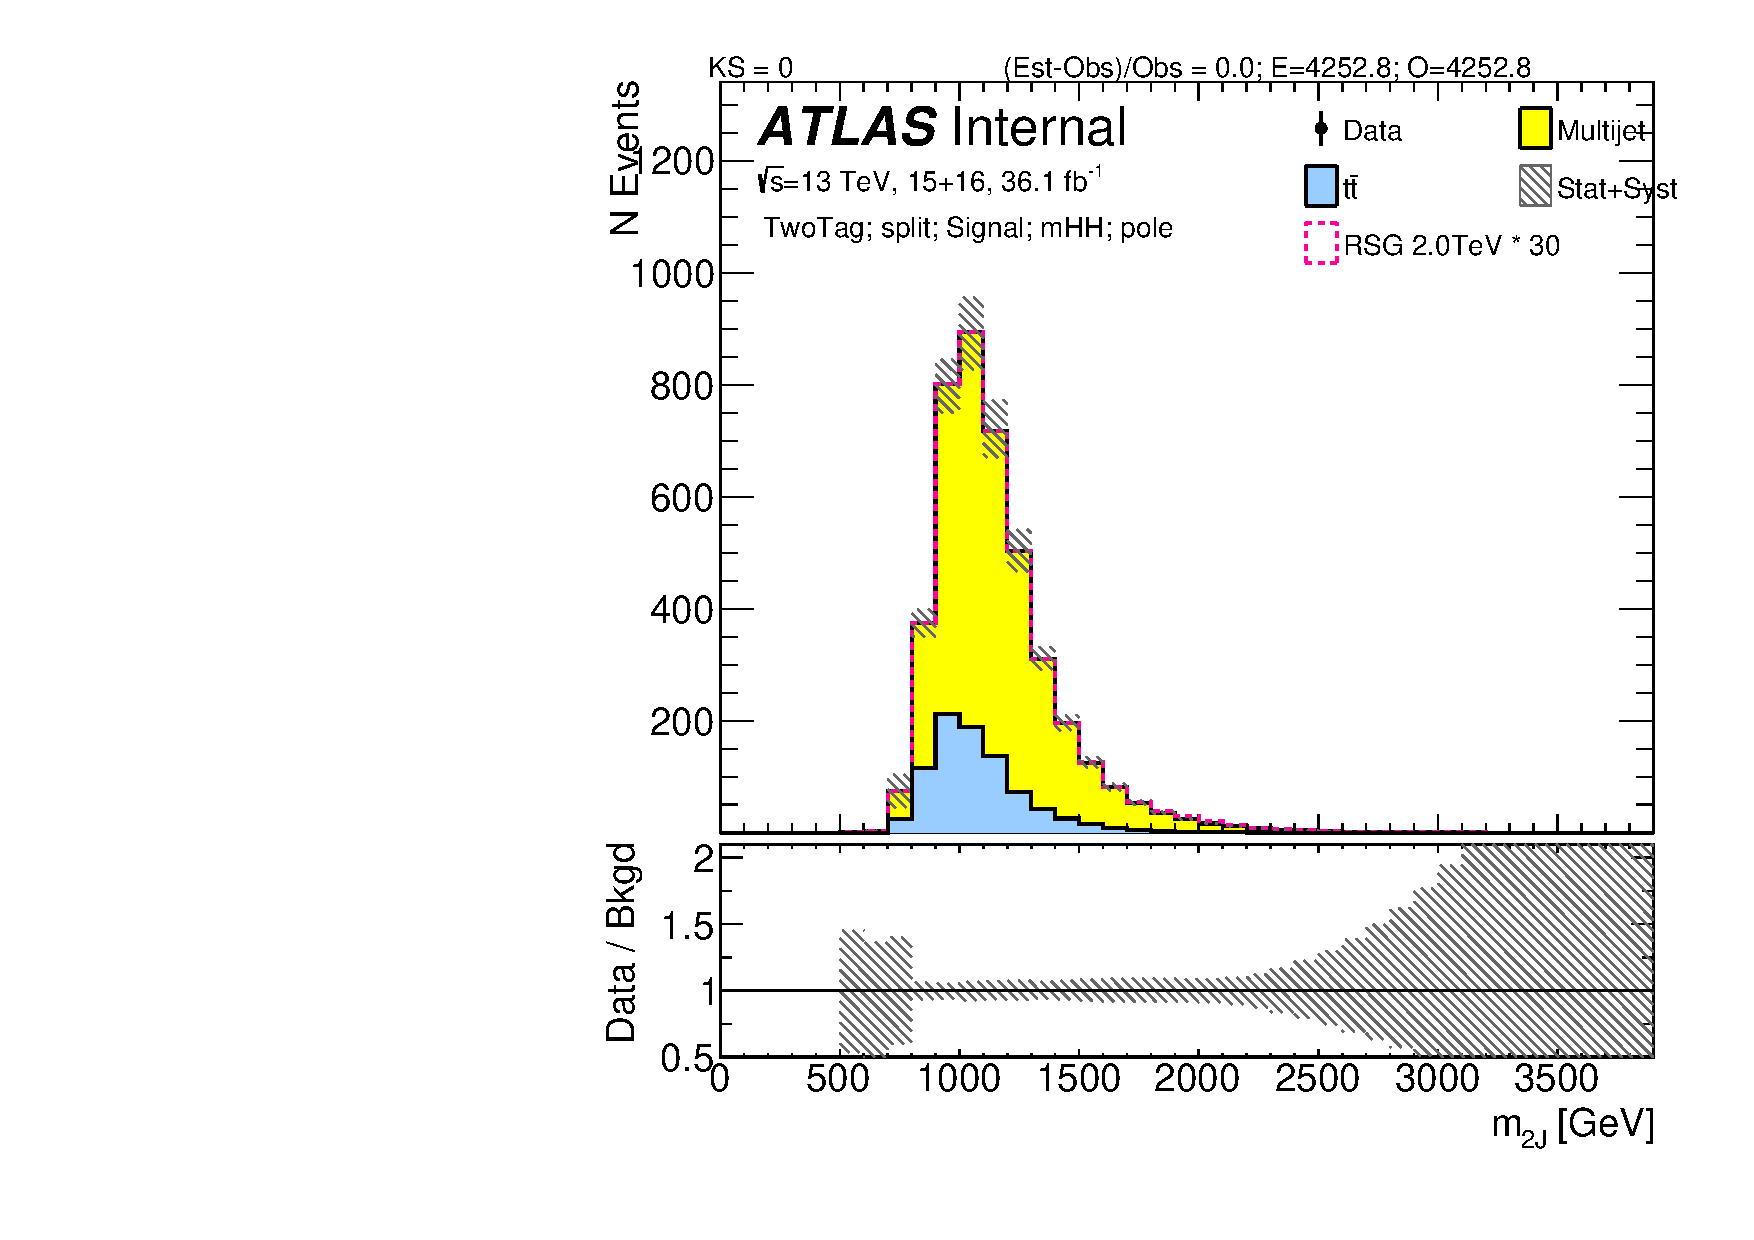
\includegraphics[angle=270, width=0.48\textwidth]{./figures/boosted/Signal_Syst/Moriond_bkg_9_TwoTag_split_Signal_mHH_pole_blind.pdf}
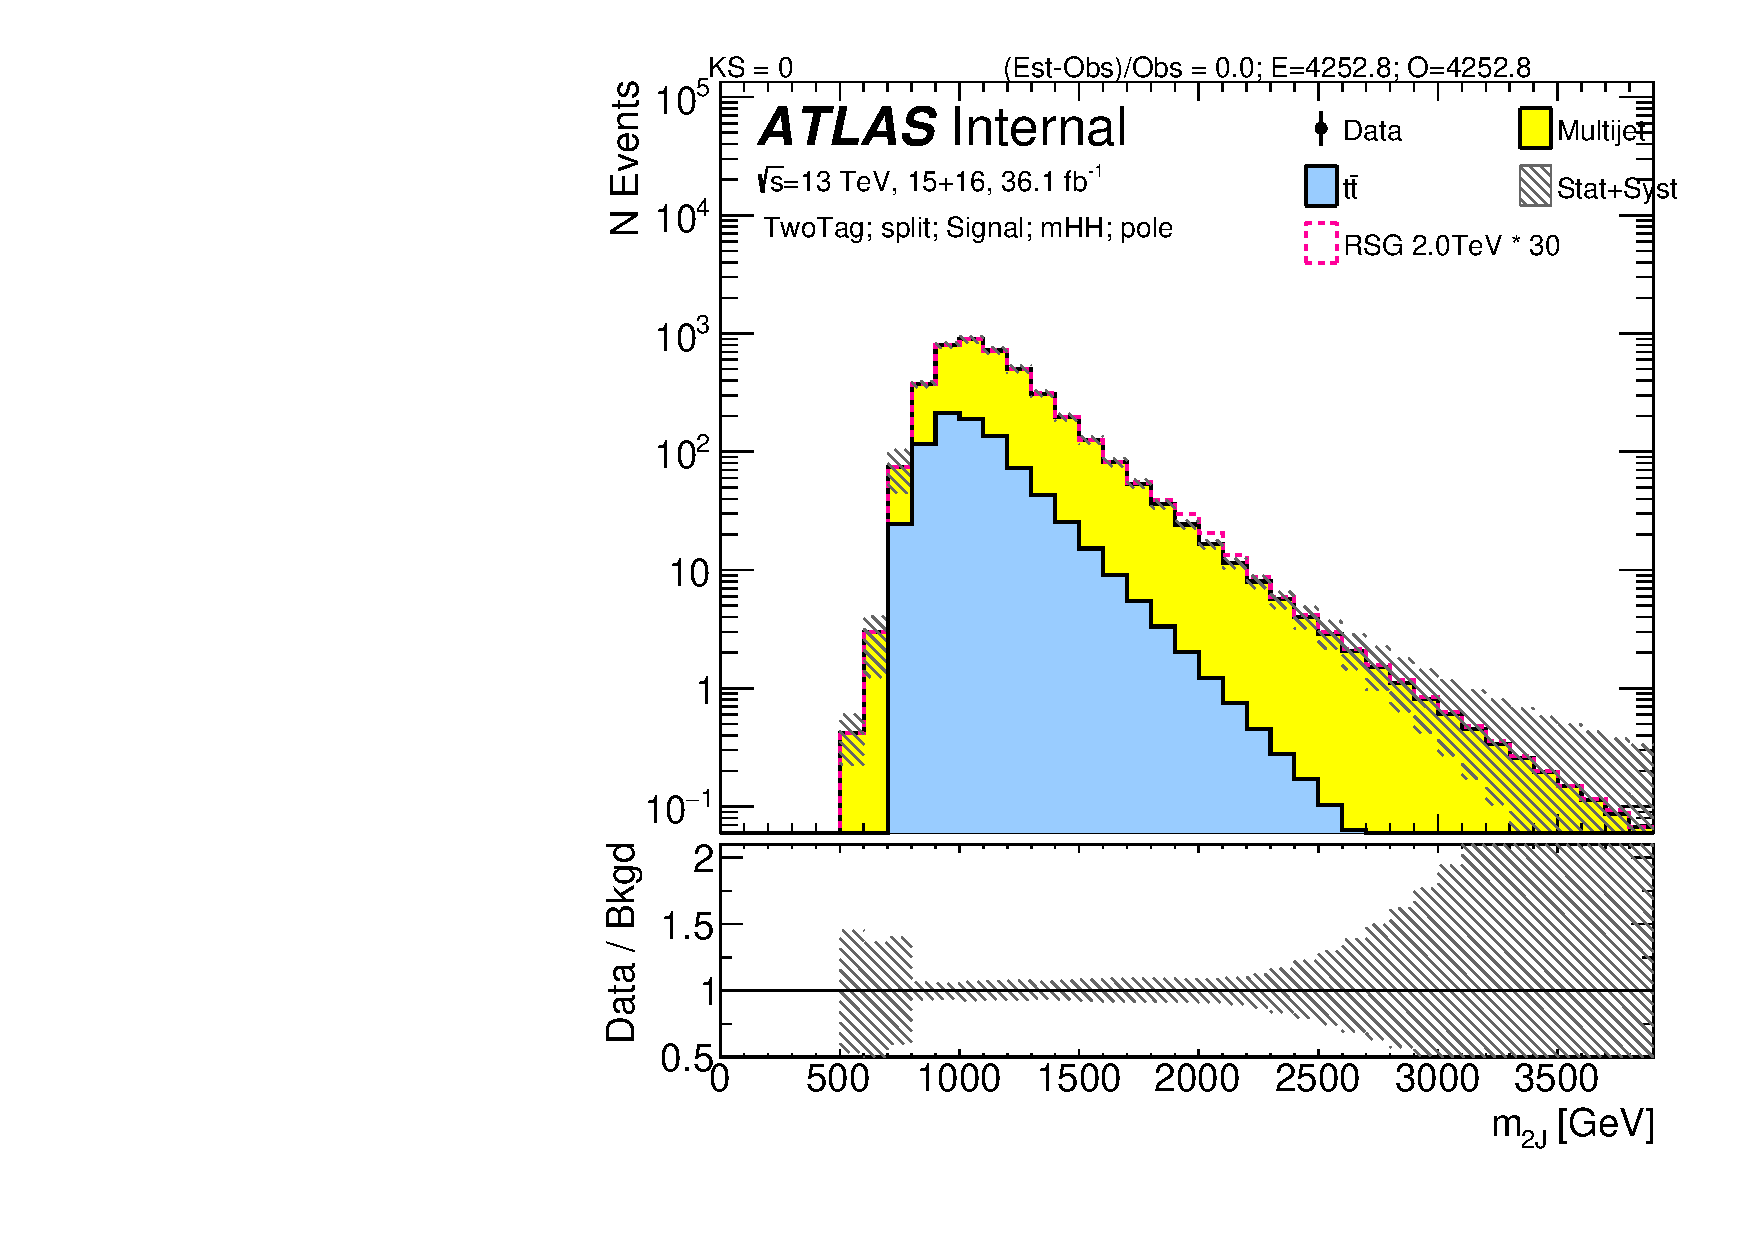
\includegraphics[angle=270, width=0.48\textwidth]{./figures/boosted/Signal_Syst/Moriond_bkg_9_TwoTag_split_Signal_mHH_pole_1_blind.pdf}
\caption{The total background estimation in $2b$s signal region, scaled mJJ, with linear scale on the left and with log scale on the right, along with total uncertainties (stats.$+$systematic) variation up and down.}
\label{fig:FinalBkg_sys-2b-pole}
\end{center}
\end{figure}
